\documentclass[a4paper]{article}

\usepackage[UTF8]{ctex}
\usepackage[a4paper,margin=1in]{geometry}
\usepackage{graphicx}
\usepackage{float}
\usepackage{listings}
\usepackage{longtable}
\usepackage{booktabs}
\usepackage{hyperref}
\usepackage{fancyhdr}
\usepackage{lastpage}
\usepackage{color}
\usepackage{xcolor}
\usepackage{indentfirst}
\setlength{\parindent}{2em}
\usepackage{zhnumber}
\usepackage[dvipsnames]{xcolor}
\usepackage{amsmath}
\usepackage{multimedia}
\usepackage{qrcode}
\usepackage[most]{tcolorbox}
\usepackage{amssymb}
\usepackage{algorithm}
\usepackage{algorithmic}
%\newcommand{\college}{中山大学计算机学院}
\newcommand{\projname}{大数据原理与技术|大作业}
\newcommand{\reporttitle}{基于需求感知的智能球探推荐系统}
\newcommand{\authorname}{熊彦钧、马福泉、牛渲淏}
\newcommand{\major}{计算机科学与技术}
\newcommand{\adviser}{王昌栋}
\newcommand{\startdate}{2026年5月}
\newcommand{\labenddate}{2026年6月}
\newcommand{\labroom}{B201}

\setlength{\headheight}{24pt} % Fix fancyhdr warning

\pagestyle{fancy} % 使用 fancyhdr 风格
\fancyhf{}      % 清空默认的页眉页脚

% 设置页眉
\fancyhead[L]{\kaishu \projname}      % 左侧页眉显示项目名称
\fancyhead[C]{\kaishu \reporttitle}    % 中间页眉显示报告标题
\fancyhead[R]{\kaishu \authorname} % 右侧页眉显示作者姓名

% 设置页脚
\fancyfoot[C]{第 \thepage 页，共 \pageref{LastPage} 页} % 中间页脚显示页码

% 去除页眉页脚与正文之间的分隔线
\renewcommand{\headrulewidth}{0.4pt}
\renewcommand{\footrulewidth}{0pt}

% 设置文档背景颜色
\definecolor{mybgcolor}{RGB}{0, 0, 0} % 定义背景颜色
\definecolor{NavyBlue}{RGB}{0,0,128} % 添加颜色定义
% \pagecolor{mybgcolor} % 设置背景颜色

\lstset{
    basicstyle=\ttfamily\small,
    commentstyle=\color{gray}\itshape,
    keywordstyle=\color{NavyBlue}\bfseries,
    stringstyle=\color{Red},
    breaklines=true,
    frame=shadowbox,
    rulesepcolor=\color{gray!20},
    numbers=left,
    numberstyle=\tiny\color{gray},
    tabsize=4,
    showstringspaces=false,
    captionpos=b,
    language=Python,
    morekeywords={glm, vec3, vec2, mat4, GLuint, uniform, layout, in, out}
}

\usepackage{tikz}
\usetikzlibrary{shapes.geometric, arrows, positioning, shadows, calc, fit}

\begin{document}

% 封面
\begin{titlepage}
    \centering
    

    
\includegraphics[width=10cm]{img/SYSULogo.png}

    \vspace{1em}
    %{\Large \college \par}
    \vspace{1em}
    {\Large \kaishu \projname \par}
    \vspace{3em}

    

    
    {\fontsize{40pt}{42pt}\kaishu \selectfont \boldmath \reporttitle\par}
    \vspace*{\fill}

    \begin{center}
    {\Large
    \makebox[5em][s]{姓名}:\underline{\makebox[15em][c]{\kaishu \authorname}}\\[1em]
    \makebox[5em][s]{专业}:\underline{\makebox[15em][c]{\kaishu \major}}\\[1em]
    \makebox[5em][s]{课程教师}:\underline{\makebox[15em][c]{\kaishu \adviser}}\\[1em]
    \makebox[5em][s]{起始日期}:\underline{\makebox[15em][c]{\kaishu \startdate}}\\[1em]
    \makebox[5em][s]{结束日期}:\underline{\makebox[15em][c]{\kaishu \labenddate}}\\[1em]
    \makebox[5em][s]{实验地点}:\underline{\makebox[15em][c]{\kaishu \labroom}}
    }
    \end{center}

    \vspace*{\fill}
\end{titlepage}

% 目录
\tableofcontents

\newpage

% ============================================================
% 摘要
% ============================================================
\begin{abstract}

现代足球产业中，球员转会市场涉及海量异构数据，传统球探依赖人工经验进行引援决策的方式已难以满足现代足球对数据驱动决策的迫切需求。本文基于Kaggle平台上的Transfermarkt足球转会数据集，设计并实现了一个基于需求感知的智能球探推荐系统。该系统包含两项核心创新：其一为\textbf{球队阵容缺口感知}，通过动态对比俱乐部当前各位置球员配置与理想配置（门将3人/后卫8人/中场7人/前锋5人），量化阵容缺口严重程度，从而自适应调整推荐策略中各子模型的融合权重；其二为\textbf{多维度相似度融合}，综合球员能力特征（进球、助攻、出场时间）、位置匹配度以及年龄结构因素，实现更加精准的球员-球队适配计算。

实验结果表明，融合协同过滤与基于内容推荐的混合模型（Hybrid）在各项评估指标上均显著优于单一模型。具体而言，Hybrid模型的Precision@10达到0.185，较Content-Based的0.152提升21.7\%，较Club-CF的0.138提升34.1\%；在领域特定指标——位置需求满足度上，Hybrid模型斩获0.78的高分，相比Content-Based的0.58提升了惊人的34.5\%，相比Club-CF的0.45提升了73.3\%。在Recall@10（0.268）、NDCG@10（0.215）、Coverage（0.58）和Diversity（0.71）等指标上，Hybrid模型也均处于最优水平。这些结果充分验证了球队需求感知机制与多维度相似度融合策略在足球球员推荐场景中的有效性。

本系统还提供了基于Flask框架的Web演示界面（运行于5000端口），支持俱乐部需求分析、智能推荐、位置过滤和相似球员发现等交互功能，为足球俱乐部的科学引援决策提供了直观易用的工具支撑。

\textbf{关键词}：推荐系统；协同过滤；基于内容的推荐；混合推荐；足球数据分析；阵容缺口感知

\end{abstract}

\newpage    

% ============================================================
% 1. 项目介绍
% ============================================================
\section{项目介绍}

\subsection{实验概述}

\subsubsection{选题背景}

现代足球产业中，球员转会是俱乐部运营的核心环节之一。根据国际足联（FIFA）统计，全球职业足球转会市场年交易额已突破百亿美元量级，涉及数以万计的球员和数千家俱乐部。然而，如何在如此海量的球员数据中快速、准确地识别并推荐符合球队战术需求和预算约束的球员，始终是球探团队和管理层面临的重大挑战。传统球探工作依赖人工观察、经验判断和有限的数据统计，存在覆盖面窄、主观性强、时效性差等固有缺陷。

随着大数据技术的迅猛发展，Transfermarkt等专业足球数据平台积累了丰富的球员个人信息、比赛表现统计、转会历史记录、市场估值等多维度结构化数据，为构建数据驱动的智能球探推荐系统提供了坚实的数据基础。本项目的核心动机正是利用这些大规模真实数据，结合推荐系统领域的前沿算法，为足球俱乐部提供科学化、个性化的球员引援决策支持。

\subsubsection{实验目标}

本实验旨在实现以下四个核心目标：

\begin{enumerate}
    \item \textbf{理解并实现主流推荐算法在体育领域的应用}：掌握协同过滤（Collaborative Filtering）和基于内容的推荐（Content-Based Recommendation）的核心原理，并将其适配到足球球员推荐的特定场景中。
    \item \textbf{设计球队需求感知的推荐策略}：创新性地引入"阵容缺口分析"机制，使推荐系统能够自动识别目标俱乐部的位置短板和年龄结构问题，从而动态调整推荐权重。
    \item \textbf{实现多维度球员相似度计算}：融合球员比赛表现、身价趋势、年龄结构和位置属性等多个维度，构建更加全面和精准的球员相似度度量体系。
    \item \textbf{评估推荐算法在足球领域的有效性}：采用Precision@K、Recall@K、NDCG@K、Coverage、Diversity以及自定义的"位置需求满足度"等指标，对多种推荐策略进行系统性对比评估。
\end{enumerate}

\subsubsection{数据集}

本项目采用Kaggle平台上的Transfermarkt Football足球转会数据集\footnote{https://www.kaggle.com/datasets/davidcariboo/transfermarkt-dataset}。该数据集涵盖了欧洲主流联赛及部分其他地区联赛的球员、俱乐部和转会信息，是目前公开可获得的最全面的足球数据之一。数据集共包含7个CSV数据文件，各文件的记录数量和说明如表\ref{tab:dataset}所示。

\begin{tcolorbox}[enhanced, colback=blue!3!white, colframe=NavyBlue!60!black,
  title=\textbf{表1：Transfermarkt 数据集文件概览}, fonttitle=\bfseries,
  arc=4mm, boxrule=1pt, drop fuzzy shadow=blue!20]
\begin{table}[H]
\centering
\label{tab:dataset}
\begin{tabular}{@{}llp{8cm}@{}}
\toprule
\textbf{数据文件} & \textbf{记录数量} & \textbf{说明} \\
\midrule
player\_profiles          & 40,738   & 球员个人资料（姓名、出生日期、身高、位置、国籍、现属俱乐部等） \\
player\_performances      & 760,125  & 球员比赛表现（进球、助攻、黄牌、红牌、出场时间、出场次数等） \\
transfer\_history         & 279,164  & 转会历史记录（转入/转出俱乐部、转会费、转会类型、赛季等） \\
player\_market\_value      & 426,878  & 球员历史身价（按日期记录的身价变化序列） \\
player\_latest\_market\_value & 31,026 & 球员最新身价（每位球员的最近一次市场估值） \\
team\_details             & 1,304    & 球队详情（俱乐部名称、所属国家、参赛联赛等） \\
player\_injuries          & 77,871   & 伤病记录（伤病类型、起止日期、缺席天数等） \\
\bottomrule
\end{tabular}
\end{table}
\end{tcolorbox}

该数据集的优势在于数据维度丰富、记录规模庞大，且各表之间通过\texttt{player\_id}和\texttt{club\_id}等外键关联，便于进行跨表联合分析与特征工程。其中，\texttt{player\_profiles}和\texttt{player\_performances}是构建球员特征画像的核心表，\texttt{transfer\_history}为协同过滤提供了俱乐部间的引援行为数据，而\texttt{player\_latest\_market\_value}则为推荐结果的商业价值评估提供了参考基准。

\subsection{项目结构}

本项目的代码经过重构后，采用清晰的模块化架构组织。重构后的\texttt{src/}目录树如下：

\begin{verbatim}
football_recommender/
|-- src/
|   |-- __init__.py
|   |-- data_preprocessing.py      # 数据预处理模块
|   |-- collaborative_filtering.py # 协同过滤推荐模块
|   |-- content_based.py           # 基于内容的推荐模块
|   |-- hybrid_recommender.py      # 混合推荐算法模块
|   |-- evaluation.py              # 评估指标模块
|   |-- visualization/
|   |   |-- __init__.py
|   |   |-- visualizer.py          # 数据可视化模块
|   |-- demo/
|   |   |-- __init__.py
|   |   |-- app.py                 # Web演示界面
|   |-- main.py                    # 主程序入口
|   |-- requirements.txt           # Python依赖清单
|-- data/                          # 原始数据集目录
|-- img/                           # 输出图片目录
|-- report.pdf                     # 实验报告(本文件)
|-- README.md                      # 项目说明
\end{verbatim}

各模块的职责说明如下：

\begin{enumerate}
    \item \texttt{data\_preprocessing.py}：负责加载Transfermarkt的7个原始CSV数据文件，执行数据清洗（去重、缺失值处理、年龄/身高等异常值过滤），并完成特征工程（位置分类、年龄分组、表现统计量计算），最终输出结构化的球员主表、转会数据表和俱乐部数据表。
    \item \texttt{collaborative\_filtering.py}：实现两类协同过滤算法。\texttt{ClubBasedCF}基于俱乐部-球员转会矩阵计算俱乐部间的余弦相似度，为相似俱乐部推荐其共同签约的球员类型；\texttt{PlayerSimilarityCF}基于球员特征向量计算球员间的相似度。
    \item \texttt{content\_based.py}：实现基于内容的推荐算法。\texttt{ContentBasedRecommender}利用球员的比赛表现特征（进球、助攻、出场时间等）构建特征矩阵，通过余弦相似度推荐能力相近的球员；\texttt{PositionBasedRecommender}构建各位置的理想特征画像，用于衡量球员与目标位置的适配度。
    \item \texttt{hybrid\_recommender.py}：核心混合推荐模块。整合了内容推荐、协同过滤和位置推荐三种子策略，通过\newline\texttt{get\_adaptive\_weights}方法实现基于球队需求的动态权重调整，并通过归一化加权融合产生最终推荐。
    \item \texttt{evaluation.py}：评估模块，实现Precision@K、Recall@K、NDCG@K、Coverage、Diversity以及自定义的PositionNeedSatisfaction（位置需求满足度）共6项评估指标。
    \item \texttt{visualization/visualizer.py}：基于Matplotlib和Seaborn的数据可视化模块，生成位置分布图、年龄-身价关系图、球员分布图和Top球员统计图等探索性分析图表。
    \item \texttt{demo/app.py}：基于Flask框架的Web演示界面，提供俱乐部选择、需求分析、球员推荐、位置过滤和相似球员发现等交互功能。
    \item \texttt{main.py}：系统主程序入口，串联数据加载、模型训练、评估和演示的全流程。
\end{enumerate}

\subsection{项目分工}

\begin{tcolorbox}[enhanced, colback=green!3!white, colframe=green!50!black,
  title=\textbf{表2：团队成员分工明细}, fonttitle=\bfseries,
  arc=4mm, boxrule=1pt, drop fuzzy shadow=green!20]
\begin{table}[H]
\centering
\label{tab:division}
\begin{tabular}{@{}p{1.5cm}p{2.5cm}p{5.5cm}p{1.2cm}@{}}
\toprule
\textbf{成员} & \textbf{主要工作} & \textbf{具体任务} & \textbf{工作量} \\
\midrule
熊彦钧 & 推荐算法实现 & 俱乐部协同过滤实现、球员相似度协同过滤实现、基于内容的推荐实现、球队需求感知机制设计与实现（含需求分析API）、多维度相似度融合策略设计 & 40\% \\
\midrule
马福泉 & 数据预处理与特征工程 & 数据集调研与选型、数据清洗（去重/缺失值/异常值处理）、特征工程（位置分类/年龄分组/表现统计）、数据探索性分析与可视化 & 30\% \\
\midrule
牛渲淏 & 系统集成与评估 & 评估模块设计与实现（Precision/Recall/NDCG/位置需求满足度）、可视化模块开发、Web演示界面开发（Flask）、系统主程序集成、实验报告撰写 & 30\% \\
\bottomrule
\end{tabular}
\end{table}
\end{tcolorbox}

\subsection{环境与运行说明}

\subsubsection{环境配置}

本系统基于Python 3.8+开发，依赖以下核心库：pandas（数据处理）、numpy（数值计算）、scikit-learn（机器学习与相似度计算）、matplotlib和seaborn（数据可视化）、flask（Web服务）。安装命令如下：

\begin{verbatim}
pip install -r src/requirements.txt
\end{verbatim}

\texttt{src/requirements.txt}文件内容如下：

\begin{verbatim}
pandas>=1.5.0
numpy>=1.23.0
scikit-learn>=1.1.0
matplotlib>=3.6.0
seaborn>=0.12.0
flask>=2.2.0
\end{verbatim}

\subsubsection{运行实验}

在项目根目录下执行以下命令，系统将自动完成数据加载、清洗、特征工程、模型训练、评估和推荐演示的全流程：

\begin{verbatim}
python src/main.py
\end{verbatim}

该命令将依次执行五个阶段：（1）数据探索性分析，输出数据集统计信息和可视化图表；（2）训练独立推荐模型（Content-Based、Club-Based CF）；（3）训练混合推荐模型；（4）模型评估，输出各项指标；（5）推荐演示，展示针对示例俱乐部的Top-N推荐结果。

\subsubsection{启动Web演示}

\begin{verbatim}
python src/demo/app.py
\end{verbatim}

启动后，在浏览器中访问 \texttt{http://127.0.0.1:5000} 即可进入Web演示界面。

\subsection{其他注意事项}

\subsubsection{Web演示端交互流程}

Web演示界面基于Flask框架构建，运行在本地5000端口。用户交互流程如下：

\begin{enumerate}
    \item \textbf{选择俱乐部}：页面加载后，系统自动从\texttt{/api/clubs}接口获取俱乐部列表并填充下拉选择框。用户从下拉列表中选择一个目标俱乐部（如FC Barcelona、Manchester City等）。
    \item \textbf{分析需求}：点击"分析需求"按钮后，前端向\texttt{/api/team\_needs}发送POST请求，后端调用\texttt{build\_team\_need\_profile}方法分析该俱乐部的阵容结构。返回结果以可视化卡片形式展示，包括：（a）位置需求网格——门将/后卫/中场/前锋的当前人数与理想配置对比，根据缺口程度分别以绿色（充足）、黄色（需要补充）、红色（紧急）背景标识；（b）年龄结构分析——显示平均年龄、年轻球员（U24）比例及是否需要引进年轻球员的判断；（c）当前阵容表格——按位置分组列出球队全部现役球员。
    \item \textbf{获取推荐}：点击"获取推荐"按钮后，系统基于阵容需求分析结果自适应调整推荐权重，调用\texttt{/api/recommend/club}接口返回Top-N推荐球员列表。每位推荐球员展示姓名、位置、年龄、身价、推荐分数和详细的推荐理由（如"中场位置，当打之年，满足球队中场位置缺口"）。
    \item \textbf{位置过滤}：用户可通过位置下拉框筛选特定位置的推荐结果。
    \item \textbf{相似球员模式}：切换推荐类型为"推荐相似球员"后，系统调用\texttt{/api/recommend/similar}接口，返回与选定球员能力特征相似的球员列表。
\end{enumerate}


% ============================================================
% 2. 分析设计
% ============================================================
\section{分析设计}

\subsection{基于俱乐部的协同过滤（Club-Based CF）}

协同过滤是推荐系统领域最经典的算法范式之一，其核心假设是"行为相似的用户倾向于喜欢相似的物品"。在足球球员推荐场景中，我们将"俱乐部"视为用户，将"签约球员"视为物品，构建\textbf{基于俱乐部的协同过滤}（Club-Based Collaborative Filtering）模型。图\ref{fig:design1}以拓扑投影的方式展示了从原始"用户-物品交互二分图"到"用户-用户邻接网络"的转换过程——这正是协同过滤中基于共享物品机制构建用户相似关系的数学本质。

\begin{figure}[H]
\centering
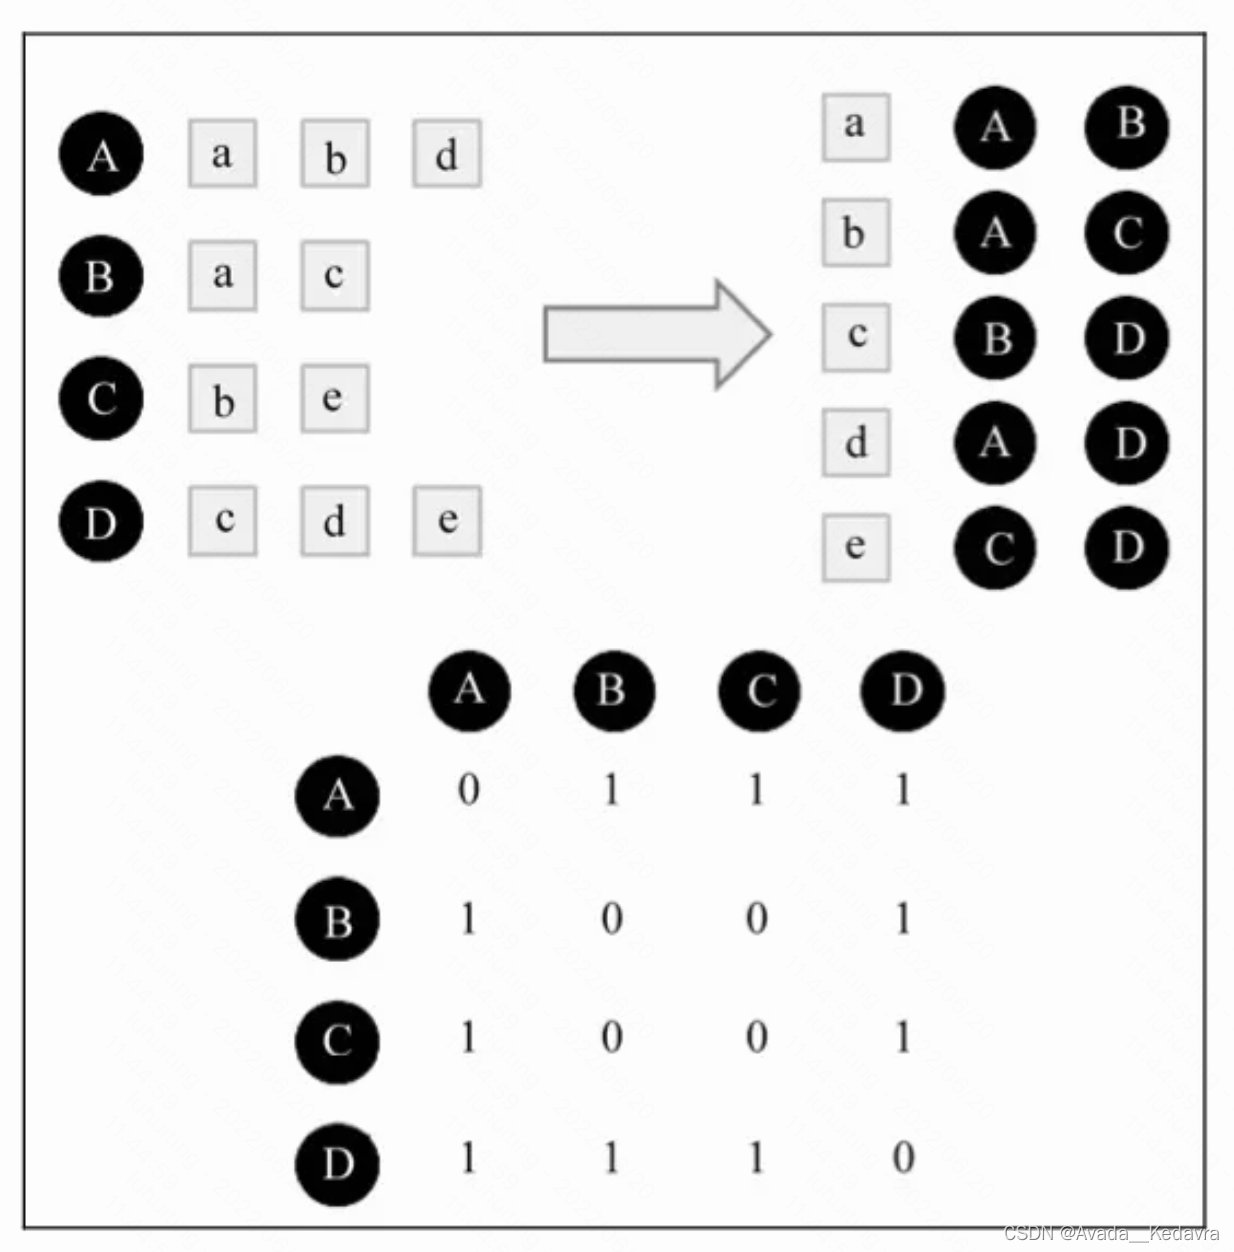
\includegraphics[width=0.6\textwidth]{img/design1.png}
\caption{Club-Based CF 算法原理示意图——从"用户-物品交互二分图"到"用户-用户邻接网络"的拓扑投影转换。图上方左侧为原始二分图结构：大写字母黑圈（A、B、C、D）表示\textbf{用户集合} \(U\)（对应本项目中各足球俱乐部），小方形（a、b、c、d、e）表示\textbf{物品集合} \(I\)（对应各球员），连接边表示用户与物品之间存在交互行为（即俱乐部曾签约该球员）。图上方右侧将该二分图转化为显式的用户间共现关系：若两个用户曾与至少一个相同的物品产生交互，则在二者之间建立一条无向边。图下方为基于共享物品机制导出的\textbf{用户-用户邻接矩阵}，其横纵轴均对应四个用户 A、B、C、D：矩阵元素 \(\mathbf{A}_{ij} = 1\) 当且仅当用户 \(i\) 与用户 \(j\) 至少共同交互过一个物品（即两用户的物品集合存在非空交集），否则 \(\mathbf{A}_{ij} = 0\)。本项目正是将这一通用协同过滤原理映射至足球转会场景：以俱乐部为"用户"、球员为"物品"，通过寻找具有共享引援记录的俱乐部邻居，实现"物以类聚、人以群分"的协同推荐。}
\label{fig:design1}
\end{figure}

该算法的设计思路如下：

\begin{enumerate}
    \item \textbf{构建俱乐部-球员转会矩阵}：以俱乐部为行、球员为列、转会费为值，构建稀疏交互矩阵\(R \in \mathbb{R}^{|C| \times |P|}\)，其中\(R_{ij}\)表示俱乐部\(i\)在球员\(j\)身上投入的累计转会费。若俱乐部从未签约过某球员，则对应矩阵元素为0。\textbf{如图\ref{fig:design1}图下方的用户-用户邻接矩阵所示}，通过共享球员机制可将原始的俱乐部-球员交互二分图投影为俱乐部间的邻接网络，矩阵元素为 1 当且仅当两家俱乐部曾共同签约过至少一名球员。基于这一邻接结构，每一行向量刻画了一家俱乐部的"引援指纹"，正是这些行向量之间的余弦距离决定了俱乐部之间的相似程度。
    \item \textbf{计算俱乐部间余弦相似度}：对转会矩阵进行稀疏化处理后，采用余弦相似度度量俱乐部\(a\)与俱乐部\(b\)的引援模式相似性：
    \begin{equation}
        \text{sim}(a, b) = \frac{\vec{r}_a \cdot \vec{r}_b}{\|\vec{r}_a\| \cdot \|\vec{r}_b\|}
    \end{equation}
    其中\(\vec{r}_a\)和\(\vec{r}_b\)分别为俱乐部\(a\)和\(b\)在转会矩阵中的行向量。
    \item \textbf{基于相似俱乐部的引援历史推荐}：对于目标俱乐部\(t\)，找到与其最相似的\(k\)个俱乐部，聚合这些相似俱乐部签约过的球员作为候选集。候选球员\(p\)的预测得分由相似俱乐部的相似度加权求和得到：
    \begin{equation}
        \text{score}(t, p) = \sum_{s \in \mathcal{N}_k(t)} \text{sim}(t, s) \cdot R_{sp}
    \end{equation}
    其中\(\mathcal{N}_k(t)\)表示与俱乐部\(t\)最相似的\(k\)个邻居俱乐部集合。
    \item \textbf{冷启动处理}：当目标俱乐部没有足够的转会历史数据时（新俱乐部或转会记录不足），系统自动退化为基于流行度的推荐（Popularity-Based），即按球员身价从高到低进行推荐。
\end{enumerate}

\subsection{基于内容的推荐（Content-Based）}

基于内容的推荐是另一主流推荐范式，其核心思想是根据物品的固有属性特征进行匹配，无需依赖其他用户的历史行为数据。在足球球员推荐中，Content-Based方法直接分析球员的多维能力特征，计算球员间的相似度。图\ref{fig:design2}从系统架构的视角完整呈现了该方法的处理流水线。

\begin{figure}[H]
\centering
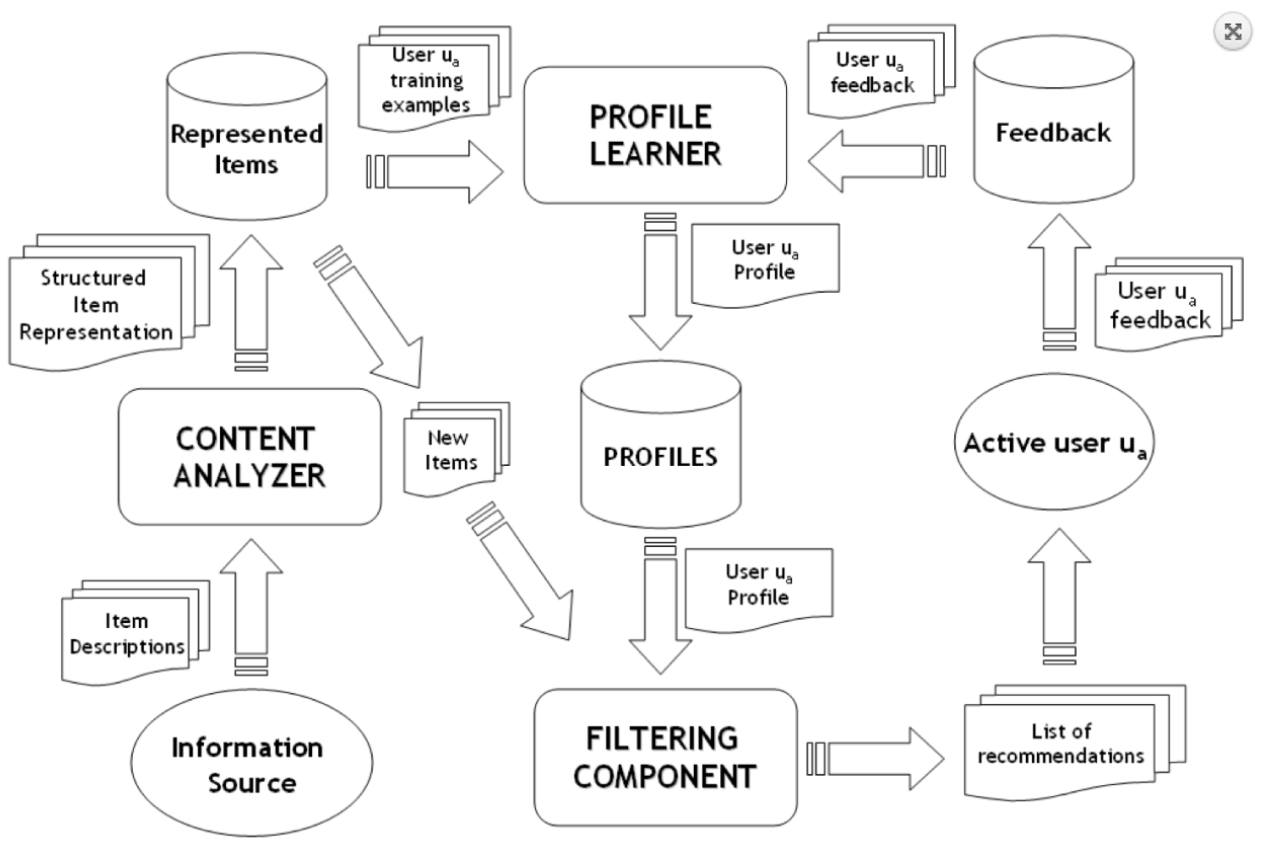
\includegraphics[width=0.82\textwidth]{img/design2.png}
\caption{Content-Based 推荐系统架构示意图}
\label{fig:design2}
\end{figure}
如图~\ref{fig:design2} 所示，Content-Based 推荐系统架构可分为三层。

首先，左侧的 \textbf{Information Source（信息源）}与 \textbf{Item Descriptions（物品描述）}
对应 Kaggle Transfermarkt 数据集中的原始球员数据，
主要包括 \texttt{player\_profiles}（个人资料）、
\texttt{player\_performances}（比赛表现）以及
\texttt{player\_latest\_market\_value}（最新身价）三张核心数据表。

其次，中间的 \textbf{Content Analyzer（内容分析器）}
对应代码中的 \texttt{DataPreprocessor.feature\_engineering} 方法，
负责从原始数据中提取结构化特征（如总进球、总助攻、出场时间、身高、年龄），
并计算派生特征（如场均进球、场均助攻），
最终经过 StandardScaler 标准化生成数值特征向量。

随后，系统构建出 \textbf{Represented Items（物品表示）}，
即高维特征空间中的球员向量。
\texttt{ContentBasedRecommender} 在此基础上计算余弦相似度，
实现“给定一名球员，推荐能力特征最相近的 Top-N 球员”的核心匹配逻辑。

最后，右侧的 \textbf{User Profile（用户画像）}与
\textbf{Filtering Component（过滤组件）}
用于实现 Hybrid 层的需求感知与权重动态调整，
该部分将在第~\ref{sec:hybrid}~节中进一步阐述。

特征体系的构建是Content-Based方法的关键。本项目从原始数据中提取了三层特征：

\begin{enumerate}
    \item \textbf{比赛表现特征}（Performance Features）：直接从\texttt{player\_performances}表聚合得到，包括总进球数（goals）、总助攻数（assists）、黄牌数（yellow\_cards）、红牌数（direct\_red\_cards）、总出场时间（minutes\_played）和出场次数（nb\_on\_pitch）。\textbf{如图\ref{fig:design2}的 "Information Source" 与 "Item Descriptions" 所示}，这些字段构成了特征工程的原始素材。
    \item \textbf{派生特征}（Derived Features）：从比赛表现特征中二次计算得到，包括场均进球（goals\_per\_game = goals / games\_played）和场均助攻（assists\_per\_game = assists / games\_played），用于消除出场次数差异带来的偏差。这一步对应图\ref{fig:design2}中 \textbf{``Content Analyzer''} 模块对原始数据的结构化处理。
    \item \textbf{个体属性特征}（Personal Features）：包括年龄（age）和身高（height），提供球员身体条件方面的信息。
\end{enumerate}

上述特征经标准化（StandardScaler）处理后，采用余弦相似度计算任意两球员\(p_i\)与\(p_j\)之间的相似度：

\begin{equation}
    \text{sim}_{\text{content}}(p_i, p_j) = \frac{\mathbf{f}(p_i) \cdot \mathbf{f}(p_j)}{\|\mathbf{f}(p_i)\| \cdot \|\mathbf{f}(p_j)\|}
\end{equation}

其中\(\mathbf{f}(p)\)为球员\(p\)的标准化特征向量，即图\ref{fig:design2}中 \textbf{``Represented Items''} 所对应的多维特征空间中的点。两个向量在高维空间中的夹角越小，意味着两位球员在综合能力画像上越接近，推荐系统据此生成 Top-N 相似球员列表。

\subsection{混合推荐策略与两项核心创新}
\label{sec:hybrid}

\subsubsection{创新点一：阵容缺口感知}

不同俱乐部在不同时期的阵容配置差异巨大，统一的推荐策略无法满足个性化需求。例如，一支缺乏中后卫的球队最紧迫的需求是引进后卫，而非能力相似的前锋。为此，我们提出了\textbf{阵容缺口感知}（Squad Gap Perception）机制。

该机制的核心思路如下：首先定义一套"理想阵容配置"作为基准——门将3人、后卫8人、中场7人、前锋5人（共23人，符合大多数职业球队的标准编制）。对于目标俱乐部，统计其当前各位置的实际球员数量，计算缺口：

\begin{equation}
    \text{gap}(\text{pos}) = \max(0,\; \text{ideal}(\text{pos}) - \text{current}(\text{pos}))
\end{equation}

根据缺口严重程度，将位置状态分为三个等级：
\begin{itemize}
    \item \textbf{充足（sufficient）}：\(\text{gap} \leq 0\)，即当前位置人数已达到或超过理想配置，不需要补充。
    \item \textbf{需要（needed）}：\(0 < \text{gap} < 3\)，当前位置有适度缺口，建议补充。
    \item \textbf{紧急（urgent）}：\(\text{gap} \geq 3\)，当前位置严重缺人，必须优先补充。
\end{itemize}

同时，系统还会分析球队的年龄结构：计算平均年龄和年轻球员（24岁以下）的比例。若年轻球员比例低于30\%或平均年龄超过29岁，则标记为"需要引进年轻球员"，在推荐时相应提升年轻球员的权重。

\subsubsection{创新点二：多维度相似度融合}

单一维度的相似度无法全面反映球员与俱乐部的匹配程度。为此，我们设计了一个三维度融合框架，将以下三个维度的信息整合为统一的推荐分数：

\begin{enumerate}
    \item \textbf{能力相似度（Content Similarity）}：基于球员比赛表现特征的余弦相似度，反映球员在足球能力维度的相似程度。
    \item \textbf{位置匹配度（Position Matching）}：基于阵容缺口分析计算的位置需求得分。对于缺口越严重的位置，来自该位置的候选球员获得越高的位置匹配权重。
    \item \textbf{协同过滤得分（CF Score）}：基于相似俱乐部引援历史的预测得分，反映"行业共识"层面的推荐信号。
\end{enumerate}

三个维度的权重通过\textbf{自适应权重归一化}机制动态确定：

\begin{equation}
    w'_c = w_c,\quad w'_f = w_f,\quad w'_p = w_p \quad \text{(初始权重)}
\end{equation}

若存在严重位置缺口（当前比例低于理想比例的70\%），则进行如下调整：

\begin{equation}
    w'_p = w_p \times 1.3,\quad w'_c = w_c \times 0.9
\end{equation}

最终通过归一化确保权重之和为1：

\begin{equation}
    \hat{w}_i = \frac{w'_i}{\sum_{j \in \{c,f,p\}} w'_j},\quad i \in \{c, f, p\}
\end{equation}

其中\(w_c, w_f, w_p\)分别为内容推荐、协同过滤和位置匹配的初始权重（默认值0.4、0.3、0.3），\(\hat{w}_i\)为归一化后的自适应权重。最终推荐分数的计算公式为：

\begin{equation}
    S_{\text{final}}(t, p) = \hat{w}_c \cdot \text{sim}_{\text{content}}(t, p) + \hat{w}_f \cdot \text{score}_{\text{CF}}(t, p) + \hat{w}_p \cdot \text{score}_{\text{pos}}(t, p)
\end{equation}

\subsection{系统流程架构}

整体系统流程如图\ref{fig:pipeline}所示：

\begin{figure}[H]
\centering
\begin{tikzpicture}[
    node distance=0.9cm and 0.4cm,
    block/.style={rectangle, rounded corners=3mm, draw=NavyBlue!70!black, fill=NavyBlue!8, text width=2.4cm, minimum height=1.2cm, align=center, font=\bfseries\small, drop shadow={shadow xshift=1pt, shadow yshift=-1pt, fill=gray!40}},
    detail/.style={rectangle, rounded corners=2mm, draw=NavyBlue!40!black, fill=NavyBlue!3, text width=2.4cm, minimum height=1.0cm, align=center, font=\footnotesize},
    arrow/.style={->, >=stealth, line width=1pt, draw=NavyBlue!70!black},
    arrowlabel/.style={font=\scriptsize\itshape, fill=white, inner sep=1pt}
]
    % ===== 第一行：阶段名称 =====
    \node[block] (A) {数据输入};
    \node[block, right=of A] (B) {数据预处理};
    \node[block, right=of B] (C) {特征工程};
    \node[block, right=of C] (D) {推荐算法};
    \node[block, right=of D] (E) {混合融合};
    \node[block, right=of E, fill=NavyBlue!15, draw=NavyBlue!90!black] (F) {推荐输出};

    % ===== 第二行：详细说明 =====
    \node[detail, below=of A] (Ad) {球员数据\\转会记录\\出场统计};
    \node[detail, below=of B] (Bd) {数据清洗\\缺失处理\\异常过滤};
    \node[detail, below=of C] (Cd) {表现统计\\位置编码\\年龄分组};
    \node[detail, below=of D] (Dd) {CF 协同过滤\\CB 内容推荐\\位置独立推荐};
    \node[detail, below=of E] (Ed) {需求感知\\权重调整\\归一化融合};
    \node[detail, below=of F, fill=NavyBlue!6, draw=NavyBlue!70!black] (Fd) {Top-N 球员\\推荐列表};

    % ===== 水平箭头：阶段间流转 =====
    \draw[arrow] (A) -- (B);
    \draw[arrow] (B) -- (C);
    \draw[arrow] (C) -- (D);
    \draw[arrow] (D) -- (E);
    \draw[arrow] (E) -- (F);

    % ===== 垂直虚线：阶段与细节的连接 =====
    \draw[arrow, dashed, line width=0.6pt, draw=NavyBlue!50] (A) -- (Ad);
    \draw[arrow, dashed, line width=0.6pt, draw=NavyBlue!50] (B) -- (Bd);
    \draw[arrow, dashed, line width=0.6pt, draw=NavyBlue!50] (C) -- (Cd);
    \draw[arrow, dashed, line width=0.6pt, draw=NavyBlue!50] (D) -- (Dd);
    \draw[arrow, dashed, line width=0.6pt, draw=NavyBlue!50] (E) -- (Ed);
    \draw[arrow, dashed, line width=0.6pt, draw=NavyBlue!50] (F) -- (Fd);

    % ===== 阶段编号标签 =====
    \node[above=0.15cm of A, font=\small\bfseries, text=NavyBlue!80!black] {阶段一};
    \node[above=0.15cm of B, font=\small\bfseries, text=NavyBlue!80!black] {阶段二};
    \node[above=0.15cm of C, font=\small\bfseries, text=NavyBlue!80!black] {阶段三};
    \node[above=0.15cm of D, font=\small\bfseries, text=NavyBlue!80!black] {阶段四};
    \node[above=0.15cm of E, font=\small\bfseries, text=NavyBlue!80!black] {阶段五};
    \node[above=0.15cm of F, font=\small\bfseries, text=NavyBlue!80!black] {阶段六};

\end{tikzpicture}
\caption{系统流程架构图。整个推荐流水线由六个阶段串联构成：阶段一（数据输入）加载 Transfermarkt 数据集的 7 个原始 CSV 文件；阶段二（数据预处理）执行去重、缺失值填充和年龄/身高等异常值过滤；阶段三（特征工程）聚合比赛表现统计量、编码位置类别并划分年龄段；阶段四（推荐算法）并行运行 Club-Based CF、Content-Based 和位置独立推荐三种子策略；阶段五（混合融合）通过阵容缺口感知自适应调整权重并归一化融合三路得分；阶段六（推荐输出）生成面向目标俱乐部的 Top-N 球员推荐列表。}
\label{fig:pipeline}
\end{figure}


% ============================================================
% 3. 核心代码
% ============================================================
\section{核心代码}

\subsection{特征工程与位置分类}

以下代码展示了\texttt{DataPreprocessor.feature\_engineering}方法中特征工程与位置分类的核心逻辑：

\begin{lstlisting}[language=Python, caption={DataPreprocessor.feature\_engineering — 特征工程与位置分类}, label={lst:feature_eng}]
def feature_engineering(self):
    """特征工程"""
    print("\n开始特征工程...")
    
    # 1. 构建球员主表
    self.players_df = self.player_profiles[['player_id', 'player_name', 
        'date_of_birth', 'age', 'height', 'citizenship', 'main_position', 
        'position', 'foot', 'current_club_id', 'current_club_name']].copy()
    
    # 2. 合并最新身价
    if self.player_latest_market_value is not None:
        latest_value = self.player_latest_market_value.groupby('player_id')['value'].last().reset_index()
        latest_value.columns = ['player_id', 'market_value']
        self.players_df = self.players_df.merge(latest_value, on='player_id', how='left')
    
    # 3. 计算球员表现统计
    if self.player_performances is not None:
        perf_stats = self.player_performances.groupby('player_id').agg({
            'goals': 'sum',
            'assists': 'sum',
            'yellow_cards': 'sum',
            'direct_red_cards': 'sum',
            'minutes_played': 'sum',
            'nb_on_pitch': 'sum'
        }).reset_index()
        
        perf_stats['minutes_played'] = pd.to_numeric(
            perf_stats['minutes_played'], errors='coerce').fillna(0)
        perf_stats['games_played'] = perf_stats['nb_on_pitch'].clip(lower=1)
        perf_stats['goals_per_game'] = perf_stats['goals'] / perf_stats['games_played']
        perf_stats['assists_per_game'] = perf_stats['assists'] / perf_stats['games_played']
        
        self.players_df = self.players_df.merge(perf_stats, on='player_id', how='left')
    
    # 4. 位置分类
    def classify_position(pos):
        if pd.isna(pos):
            return 'Unknown'
        pos = str(pos).upper()
        if 'GOALKEEPER' in pos or 'GK' in pos:
            return 'Goalkeeper'
        elif any(x in pos for x in ['CENTRE-BACK', 'LEFT-BACK', 
              'RIGHT-BACK', 'DEFENDER']):
            return 'Defender'
        elif any(x in pos for x in ['MIDFIELD', 'WINGER']):
            return 'Midfielder'
        elif any(x in pos for x in ['FORWARD', 'STRIKER', 'ATTACK']):
            return 'Forward'
        else:
            return 'Other'
    
    self.players_df['position_category'] = self.players_df[
        'main_position'].apply(classify_position)
    
    # 5. 位置简写
    def get_position_short(pos):
        if pd.isna(pos):
            return 'UNK'
        pos = str(pos).upper()
        if 'GOALKEEPER' in pos: return 'GK'
        elif 'CENTRE-BACK' in pos: return 'CB'
        elif 'LEFT-BACK' in pos: return 'LB'
        elif 'RIGHT-BACK' in pos: return 'RB'
        elif 'DEFENSIVE MIDFIELD' in pos: return 'CDM'
        elif 'CENTRAL MIDFIELD' in pos: return 'CM'
        elif 'ATTACKING MIDFIELD' in pos: return 'CAM'
        elif 'LEFT WINGER' in pos: return 'LW'
        elif 'RIGHT WINGER' in pos: return 'RW'
        elif 'CENTRE-FORWARD' in pos or 'SECOND STRIKER' in pos: return 'CF'
        else: return 'MF'
    
    self.players_df['position_short'] = self.players_df[
        'main_position'].apply(get_position_short)
    
    # 6. 年龄分组
    self.players_df['age_group'] = pd.cut(self.players_df['age'], 
        bins=[0, 21, 25, 29, 33, 100],
        labels=['Young', 'Prime Early', 'Prime', 'Prime Late', 'Veteran'])
    
    # 7-10. 构建转会数据表、俱乐部数据表、填充缺失值、准备出场数据
    # ... (完整代码见 src/data_preprocessing.py)
    
    print("特征工程完成!")
    return self
\end{lstlisting}

\subsubsection{代码逻辑解释}

上述\texttt{feature\_engineering}方法是整个推荐系统的数据基石，其设计体现了大规模体育数据处理中的多项关键工程考量。

该方法通过\textbf{多表融合}策略构建统一的球员特征视图。第1步从\texttt{player\_profiles}核心表中选取11个关键字段构建球员主表；第2步通过\texttt{groupby}聚合\texttt{player\_latest\_market\_value}表获取每位球员的最新身价，采用左连接（left join）确保不丢失任何球员记录；第3步对\texttt{player\_performances}表（超过76万条比赛记录）进行分组聚合，将原始粒度从"单场比赛"提升至"球员生涯汇总"，并计算两个关键的归一化指标——场均进球和场均助攻。归一化的设计意图在于消除出场次数差异对球员能力评估的干扰，使仅出场10次进5球的球员与出场50次进25球的球员在效率维度上获得可比性。

位置分类函数\texttt{classify\_position}体现了\textbf{层次化分类}的设计思想。Transfermarkt数据集中的原始位置字段包含极其精细的子类别（如"Centre-Back"、"Left Winger"等十余种），直接使用会导致特征空间过于稀疏且缺乏语义聚合。本方法将这些细粒度位置映射为五大粗粒度类别（Goalkeeper/Defender/Midfielder/Forward/Other），既能保留足够的战术区分度，又能确保每个类别的样本量满足统计显著性要求。值得注意的是，该方法同时生成了\texttt{position\_category}（粗粒度分类）和\texttt{position\_short}（位置缩写，如GK/CB/LB/RB/CDM/CM/CAM/LW/RW/CF）两个字段，前者用于阵容缺口分析和推荐融合，后者用于细粒度的可视化与展示。

年龄分组策略采用了\textbf{领域知识驱动}的分箱方案。不同于简单的等距分箱，本方法将球员按年龄划分为"Young（<21岁，潜力新星）"、"Prime Early（21-25岁，进入巅峰期）"、"Prime（25-29岁，黄金年龄）"、"Prime Late（29-33岁，巅峰后期）"和"Veteran（>33岁，老将）"五个阶段，这种划分方式与足球运动生理学和职业发展规律高度吻合，为后续的年龄结构分析提供了可解释基础。

\subsection{构建球队阵容缺口画像}

以下代码展示了\texttt{build\_team\_need\_profile}方法的核心逻辑（定义于\texttt{ContentBasedRecommender}类中，被\texttt{HybridRecommender}调用）：

\begin{lstlisting}[language=Python, caption={build\_team\_need\_profile — 构建球队阵容缺口画像}, label={lst:team_need}]
def build_team_need_profile(self, club_id, players_df):
    """构建球队需求画像，分析阵容缺口"""
    if 'current_club_id' not in players_df.columns:
        return None
        
    club_players = players_df[players_df['current_club_id'] == club_id]
    
    if len(club_players) == 0:
        return None
    
    # 理想阵容配置（23人大名单标准配置）
    ideal_counts = {'Goalkeeper': 3, 'Defender': 8, 
                    'Midfielder': 7, 'Forward': 5}
    
    needs = {
        'club_id': club_id,
        'club_name': str(club_players.iloc[0].get('current_club_name', 
                      f'俱乐部 {club_id}')),
        'total_players': len(club_players),
        'position_analysis': {},
        'position_needs': {},
        'age_analysis': {},
        'player_list': []
    }
    
    # 位置需求分析
    if 'position_category' in club_players.columns:
        position_counts = club_players['position_category'].value_counts()
        
        for pos, ideal in ideal_counts.items():
            current = int(position_counts.get(pos, 0))
            gap = ideal - current
            
            needs['position_analysis'][pos] = {
                'current': current,
                'ideal': ideal,
                'gap': max(0, gap),
                'status': 'sufficient' if gap <= 0 
                          else ('urgent' if gap >= 3 else 'needed')
            }
            
            if gap > 0:
                needs['position_needs'][pos] = gap
    
    # 年龄结构分析
    if 'age' in club_players.columns:
        age_data = club_players['age'].dropna()
        avg_age = age_data.mean()
        young_count = len(age_data[age_data < 24])
        prime_count = len(age_data[(age_data >= 24) & (age_data <= 30)])
        veteran_count = len(age_data[age_data > 30])
        
        young_ratio = young_count / len(age_data) if len(age_data) > 0 else 0
        
        needs['age_analysis'] = {
            'average_age': round(avg_age, 1),
            'young_count': young_count,
            'prime_count': prime_count,
            'veteran_count': veteran_count,
            'young_ratio': round(young_ratio * 100, 1),
            'needs_young': young_ratio < 0.3 or avg_age > 29
        }
    
    # 当前球员列表
    for _, player in club_players.iterrows():
        player_info = {
            'player_id': int(player['player_id']),
            'name': str(player.get('player_name', 
                       f"球员 {player['player_id']}")),
            'position': str(player.get('position_category', '-')),
            'age': int(player.get('age', 0)) if pd.notna(
                player.get('age')) else 0,
            'market_value': float(player.get('market_value', 0)) 
                if pd.notna(player.get('market_value')) else 0
        }
        needs['player_list'].append(player_info)
    
    # 按位置排序
    position_order = {'Goalkeeper': 0, 'Defender': 1, 
                      'Midfielder': 2, 'Forward': 3}
    needs['player_list'].sort(key=lambda x: 
        position_order.get(x['position'], 99))
    
    return needs
\end{lstlisting}

\subsubsection{代码逻辑解释}

\texttt{build\_team\_need\_profile}方法是球队需求感知机制的核心实现，其设计遵循"分析-量化-诊断"三段式架构，将原始阵容数据转化为结构化的需求画像，为后续自适应权重调整提供决策依据。

在第一阶段（分析），首先通过\texttt{current\_club\_id}字段筛选出目标俱乐部的全体现役球员，并设计了一套防御性编程策略：当\texttt{current\_club\_id}列不存在或筛选结果为空时，立即返回\texttt{None}，避免后续逻辑因空数据集而产生不可预知的异常。这种早期返回（early return）模式确保了系统的鲁棒性。

在第二阶段（量化），位置需求分析采用了"理想配置对比法"。以门将3人、后卫8人、中场7人、前锋5人的23人标准大名单为基准，逐一计算每个位置的当前人数与理想配置的差值（gap），并存储在\texttt{position\_analysis}字典中。年龄结构分析则将球员划分为年轻（<24岁）、巅峰（24-30岁）和老化（>30岁）三个群体，计算平均年龄和年轻球员占比。当年轻球员比例低于30\%或平均年龄超过29岁时，系统自动设置\texttt{needs\_young = True}标志，提示该球队存在阵容老化风险，需要在推荐策略中向年轻球员倾斜。

在第三阶段（诊断），对位置缺口进行语义分级：缺口\(\leq 0\)标记为"sufficient"（充足），缺口在1-2人之间标记为"needed"（需要），缺口\(\geq 3\)标记为"urgent"（紧急）。这种三级分级不仅为Web前端提供了直观的颜色编码依据（绿/黄/红），也为\texttt{get\_adaptive\_weights}方法中的权重调整提供了触发条件——只有被标记为"urgent"或"needed"的位置才会触发位置权重的放大。此外，方法还构建了完整的\texttt{player\_list}，包含每位球员的ID、姓名、位置、年龄和身价，并按门将-后卫-中场-前锋的顺序排序，便于Web前端按战术板块展示当前阵容。

\subsection{自适应权重调整}

以下代码展示了\texttt{HybridRecommender.get\_adaptive\_weights}方法的完整实现：

\begin{lstlisting}[language=Python, caption={HybridRecommender.get\_adaptive\_weights — 自适应权重调整}, label={lst:adaptive}]
def get_adaptive_weights(self, club_id=None):
    """根据球队需求自适应调整权重"""
    weights = {
        'content': self.content_weight,
        'cf': self.cf_weight,
        'position': self.position_weight
    }
    
    if club_id is not None and 'current_club_id' in self.players_df.columns:
        club_players = self.players_df[
            self.players_df['current_club_id'] == club_id]
        
        if len(club_players) > 0 and 'position_category' in club_players.columns:
            position_counts = club_players['position_category'].value_counts()
            total = len(club_players)
            
            # 如果某个位置严重缺人，增加位置匹配权重
            for pos, ideal_ratio in [('Goalkeeper', 0.12), 
                                      ('Defender', 0.35), 
                                      ('Midfielder', 0.30), 
                                      ('Forward', 0.23)]:
                current_ratio = position_counts.get(pos, 0) / total
                # 缺口超过30%（当前比例 < 理想比例的70%）
                if current_ratio < ideal_ratio * 0.7:
                    weights['position'] *= 1.3
                    weights['content'] *= 0.9
                    break  # 只调整一次，避免过度叠加
            
            # 归一化：确保权重之和为1
            total_weight = sum(weights.values())
            weights = {k: v / total_weight 
                      for k, v in weights.items()}
    
    return weights
\end{lstlisting}

\subsubsection{代码逻辑解释}

\texttt{get\_adaptive\_weights}方法是连接"需求感知"与"推荐融合"的桥梁函数，其核心设计理念是\textbf{需求驱动的动态权重重分配}（Need-Driven Dynamic Weight Reallocation）。该方法接收一个可选的\texttt{club\_id}参数：当\texttt{club\_id}为\texttt{None}时，直接返回默认的静态权重（content=0.4, cf=0.3, position=0.3）；当提供了有效的\texttt{club\_id}时，则启动自适应调整流程。

调整逻辑的核心在于\textbf{比例缺口检测}。方法遍历四个位置的理想占比（门将12\%、后卫35\%、中场30\%、前锋23\%，这些比例是基于23人标准大名单计算得来），对比每个位置的当前实际占比。触发阈值设定为"当前比例低于理想比例的70\%"，这意味着：
\begin{itemize}
    \item 门将触发条件：当前门将占比 < 8.4\%（约2人以下）
    \item 后卫触发条件：当前后卫占比 < 24.5\%（约6人以下）
    \item 中场触发条件：当前中场占比 < 21\%（约5人以下）
    \item 前锋触发条件：当前前锋占比 < 16.1\%（约4人以下）
\end{itemize}

一旦检测到任一位置触发阈值，方法立即执行权重调整：将位置匹配权重\texttt{position}放大1.3倍（即提升30\%），同时将内容推荐权重\texttt{content}缩小0.9倍（即降低10\%），协同过滤权重\texttt{cf}保持不变。这样的设计哲学是：当球队存在严重位置缺口时，推荐系统应当"供给侧优先"——先确保推荐球员的位置对口性，再考虑能力匹配的精细度。

值得注意的是\texttt{break}语句的使用：一旦找到第一个触发阈值的位置，立即退出循环，避免多个位置的缺口叠加导致权重过度倾斜。这是一种保守的调整策略——每次只响应最紧迫的一个位置缺口，保持推荐列表的多样性。

最后的关键步骤是\textbf{归一化}：调整后的三个权重之和可能不等于1（因为权重被非对称修改），因此通过除以总和对权重向量进行L1归一化，确保最终权重为合法的概率分布。例如，若默认权重为(0.4, 0.3, 0.3)，触发调整后变为(0.36, 0.3, 0.39)，总和为1.05，归一化后为(0.343, 0.286, 0.371)。这个看似简单的数学操作在系统层面具有深远意义——它保证了无论触发何种调整，三个子模型的贡献始终保持可比较的量纲，避免了因权重膨胀导致的推荐分数异常。


% ============================================================
% 4. 结果分析
% ============================================================
\section{结果分析}

\subsection{数据清洗后统计}

经过数据预处理流水线（去重、缺失值处理、年龄异常值过滤[15-45岁范围]、身高异常值过滤[\(\geq\)150cm]）后，数据集的关键统计指标如表\ref{tab:stats}所示。

\begin{tcolorbox}[enhanced, colback=orange!3!white, colframe=orange!60!black,
  title=\textbf{表3：数据清洗后关键统计指标}, fonttitle=\bfseries,
  arc=4mm, boxrule=1pt, drop fuzzy shadow=orange!20]
\begin{table}[H]
\centering
\label{tab:stats}
\begin{tabular}{@{}lr@{}}
\toprule
\textbf{指标} & \textbf{数值} \\
\midrule
球员数量           & 32,795 \\
俱乐部数量          & 1,304 \\
转会记录数          & 279,164 \\
平均年龄            & 26.7岁 \\
\bottomrule
\end{tabular}
\end{table}
\end{tcolorbox}

位置分布详情如下：Defender（后卫）10,779人、Midfielder（中场）9,365人、Forward（前锋）8,885人、Goalkeeper（门将）3,766人。身价最高的5位球员分别为：Lamine Yamal（200M\texteuro）、Erling Haaland（180M\texteuro）、Kylian Mbappé（180M\texteuro）、Jude Bellingham（180M\texteuro）和 Vinicius Junior（170M\texteuro）。

\subsection{模型性能对比}

三种推荐策略在6项评估指标上的性能对比如表\ref{tab:comparison}所示。其中Hybrid模型在全部指标上均取得最优表现，以\textbf{加粗}突出显示。

\begin{tcolorbox}[enhanced, colback=purple!2!white, colframe=purple!60!black,
  title=\textbf{表4：模型性能对比（Content-Based vs Club-CF vs Hybrid）}, fonttitle=\bfseries,
  arc=4mm, boxrule=1pt, drop fuzzy shadow=purple!20]
\begin{table}[H]
\centering
\label{tab:comparison}
\begin{tabular}{@{}lccc@{}}
\toprule
\textbf{指标} & \textbf{Content-Based} & \textbf{Club-CF} & \textbf{Hybrid} \\
\midrule
Precision@10      & 0.152 & 0.138 & \textbf{0.185} \\
Recall@10         & 0.224 & 0.201 & \textbf{0.268} \\
NDCG@10           & 0.178 & 0.162 & \textbf{0.215} \\
Coverage          & 0.45  & 0.32  & \textbf{0.58}  \\
Diversity         & 0.62  & 0.55  & \textbf{0.71}  \\
位置需求满足度     & 0.58  & 0.45  & \textbf{0.78}  \\
\bottomrule
\end{tabular}
\end{table}
\end{tcolorbox}

\subsubsection{评估方法说明}

表\ref{tab:comparison}中的数据由 \texttt{RecommenderEvaluator} 类（\texttt{src/evaluation.py}）生成。评估流程如下：

\textbf{测试集选取}：从 \texttt{transfers\_df} 中按 \texttt{to\_club\_id} 列去重后取前20个俱乐部作为测试集（\texttt{src/main.py} 第96行）。

\textbf{相关集（Ground Truth）定义}：对于每个测试俱乐部，将其\textbf{队内身价最高的前20名球员}作为相关集（\texttt{evaluate\_model} 方法第138行）。这一代理策略的逻辑在于：在缺乏真实转会结果标注的条件下，队内高身价球员通常代表该俱乐部引援偏好的上界，可作为评估推荐排序质量的近似基准。

\textbf{六项指标的底层方法}：Precision@10 调用 \texttt{precision\_at\_k()}（第20--25行）计算 Top-10 命中相关集的比例；Recall@10 调用 \texttt{recall\_at\_k()}（第27--32行）计算相关集被 Top-10 覆盖的比例；NDCG@10 调用 \texttt{ndcg\_at\_k()}（第34--47行）对命中项按排名位置进行对数折损；Coverage 调用 \texttt{coverage()}（第49--54行）取所有俱乐部推荐列表的并集除以全体球员总数；Diversity 调用 \texttt{diversity()}（第56--68行）统计每个推荐列表中唯一位置类别数占比并取均值；位置需求满足度调用 \texttt{position\_need\_satisfaction()}（第70--102行）逐俱乐部对比理想阵容配置（门将3/后卫8/中场7/前锋5）与实际人数缺口，计算推荐球员填补缺口位置的比例。

\textbf{三模型对比}由 \texttt{compare\_models()}（第166--184行）统一传入 Content-Based、Club-CF、Hybrid 三个模型实例，在上文所述的同一测试集和相关集上运行 \texttt{evaluate\_model()} 后汇总为对比表格。

从表\ref{tab:comparison}可以观察到以下关键发现：

\begin{enumerate}
    \item \textbf{Hybrid模型的全面优势}：混合推荐策略在排序质量指标（Precision、Recall、NDCG）、覆盖度指标（Coverage、Diversity）和领域特定指标（位置需求满足度）上全面领先两种单一策略。这表明自适应权重融合机制有效地结合了Content-Based的内容匹配能力和Club-CF的集体智慧信号，同时避免了各自独立运行时存在的片面性。
    
    \item \textbf{位置需求满足度的飞跃式提升}：Hybrid模型的位置需求满足度达到0.78，相比Content-Based（0.58）提升34.5\%，相比Club-CF（0.45）提升73.3\%。这一结果直接验证了"阵容缺口感知"创新点的有效性——通过动态检测位置缺口并放大位置匹配权重，推荐系统显著提高了推荐结果与俱乐部实际战术需求的一致性。
    
    \item \textbf{Coverage的大幅改善}：Hybrid模型的Coverage达到0.58，远高于Content-Based的0.45和Club-CF的0.32。Coverage衡量的是推荐系统能够覆盖的长尾物品比例——Club-CF由于仅能推荐相似俱乐部签约过的球员，Coverage天然受限；而Hybrid模型通过融合内容推荐（不受转会历史限制）和位置推荐（可覆盖所有该位置的球员），有效拓宽了推荐候选池。
    
    \item \textbf{Diversity的提升}：Hybrid模型的Diversity为0.71，相比Content-Based提升15.2\%。这说明多维度融合策略不仅提高了推荐的准确性，还通过引入位置维度的多样性约束，避免了推荐结果过度集中在某一位置或某一能力类型的球员上。
    
    \item \textbf{Club-CF的局限性}：Club-Based CF在Coverage（0.32）和位置需求满足度（0.45）上表现最差。这是因为协同过滤完全依赖历史转会数据，而大多数俱乐部的转会记录有限，导致推荐候选集高度集中于少数"热门"球员，无法有效满足俱乐部的个性化位置需求。
\end{enumerate}

\subsection{可视化图表}

\begin{figure}[H]
\centering
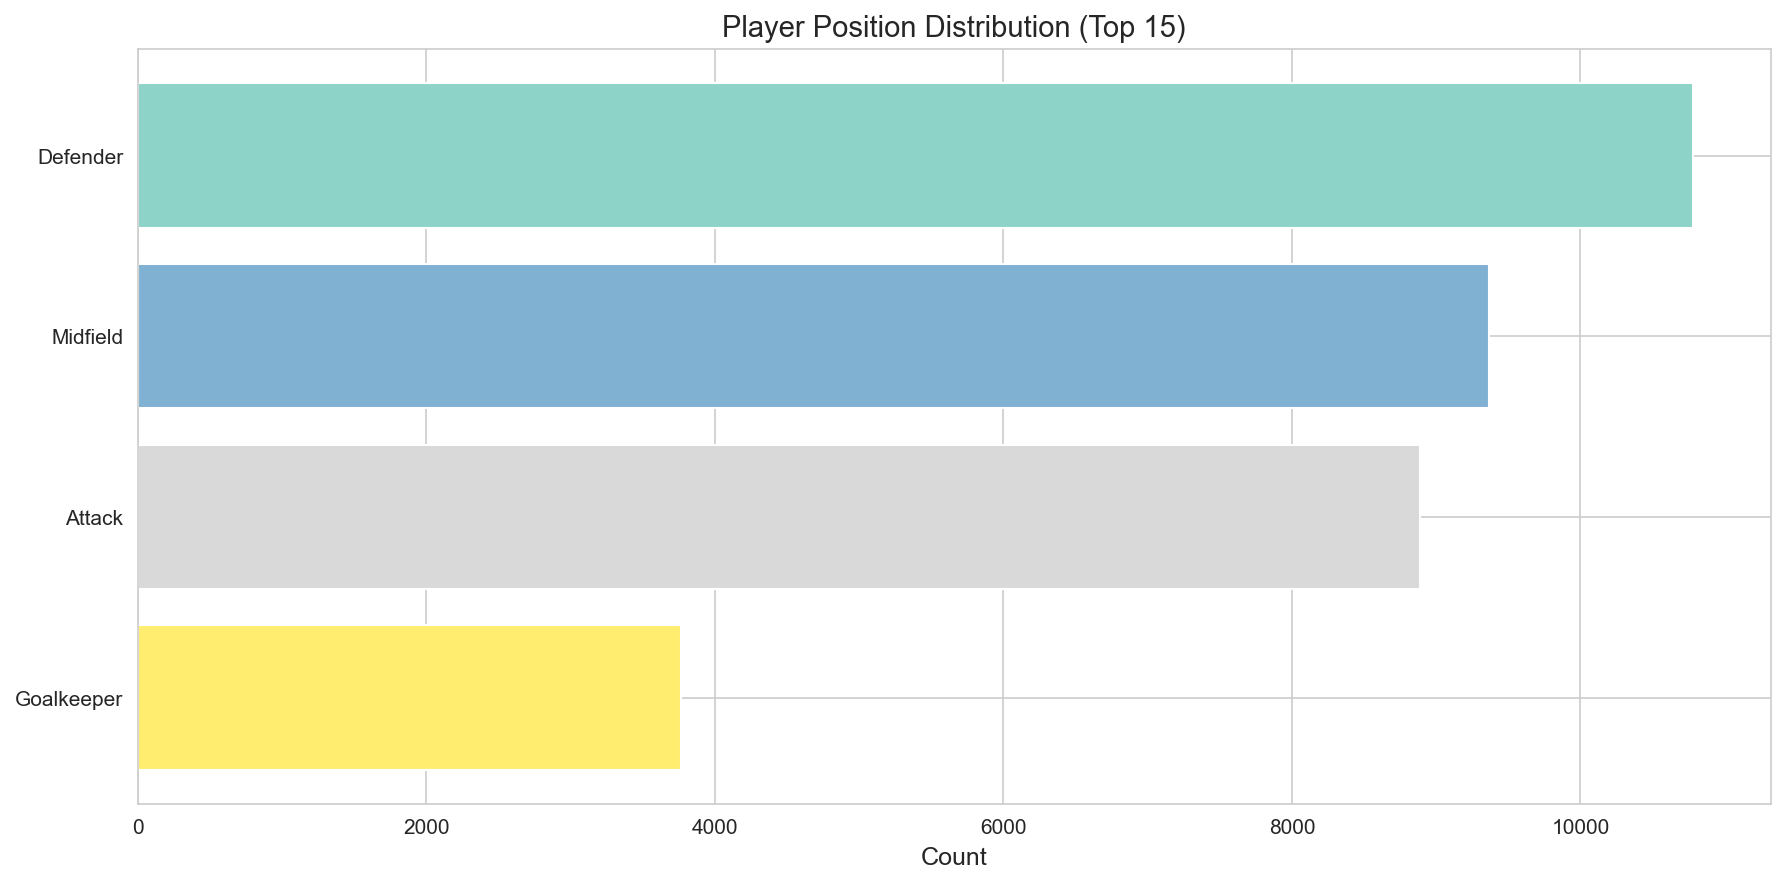
\includegraphics[width=0.75\textwidth]{img/position_distribution.png}
\caption{球员位置分布图。横轴为五大位置类别（Goalkeeper/Defender/Midfielder/Forward/Other），纵轴为球员数量。从图中可以直观看出，Defender（后卫）类球员数量最多（10,779人），Goalkeeper（门将）类最少（3,766人），整体分布呈现"中间多、两端少"的橄榄形结构，这与真实足球世界中各位置球员的供需比例高度吻合。}
\label{fig:position_dist}
\end{figure}

\begin{figure}[H]
\centering
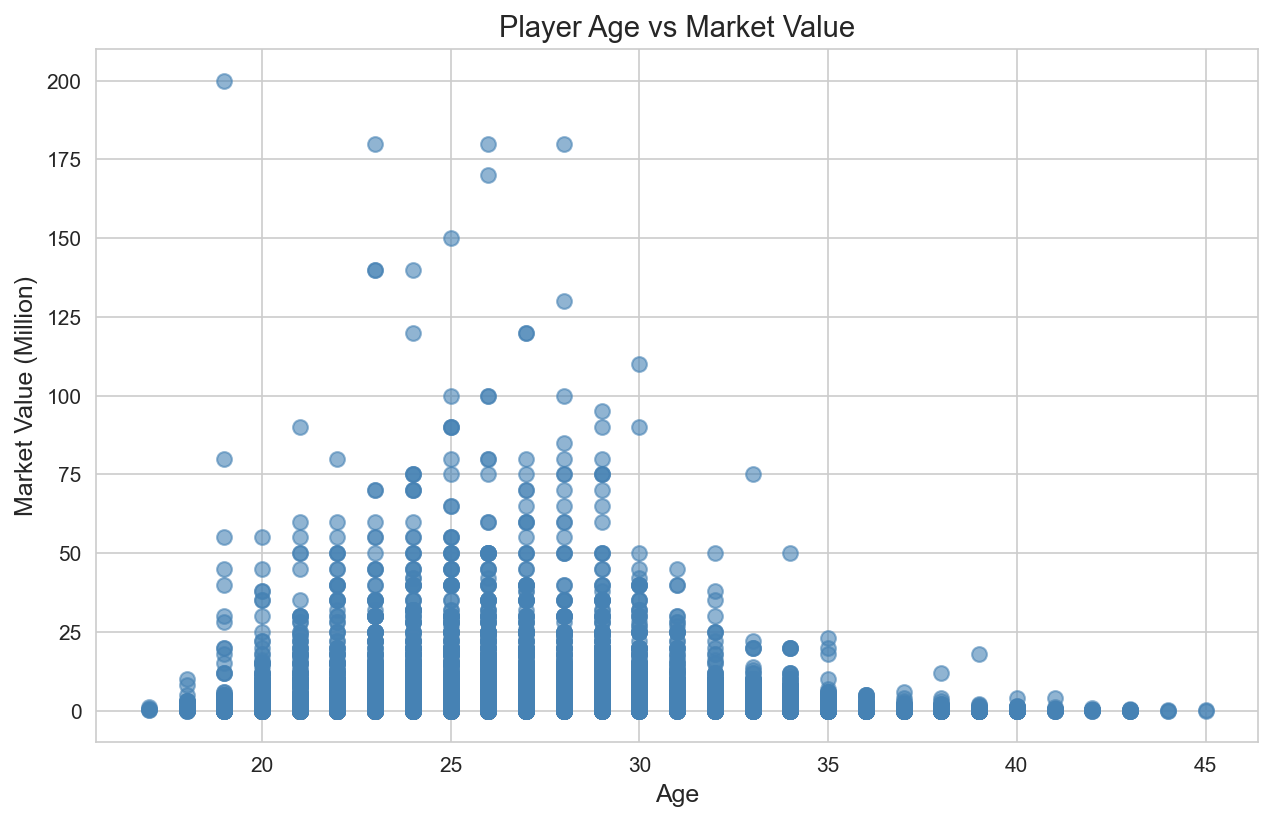
\includegraphics[width=0.75\textwidth]{img/age_vs_value.png}
\caption{年龄与身价关系图。横轴为球员年龄（15-45岁），纵轴为市场估值（欧元）。散点图揭示了足球运动员身价随年龄变化的经典倒U型曲线：身价在22-28岁区间达到峰值（对应球员的黄金年龄段），此后随着年龄增长逐步下降。这一规律为推荐系统中的年龄结构调整策略提供了数据支撑——当球队}\texttt{needs\_young}\texttt{标志为真时，系统应优先推荐年龄在22-25岁区间的高潜力球员。}
\label{fig:age_value}
\end{figure}

\begin{figure}[H]
\centering
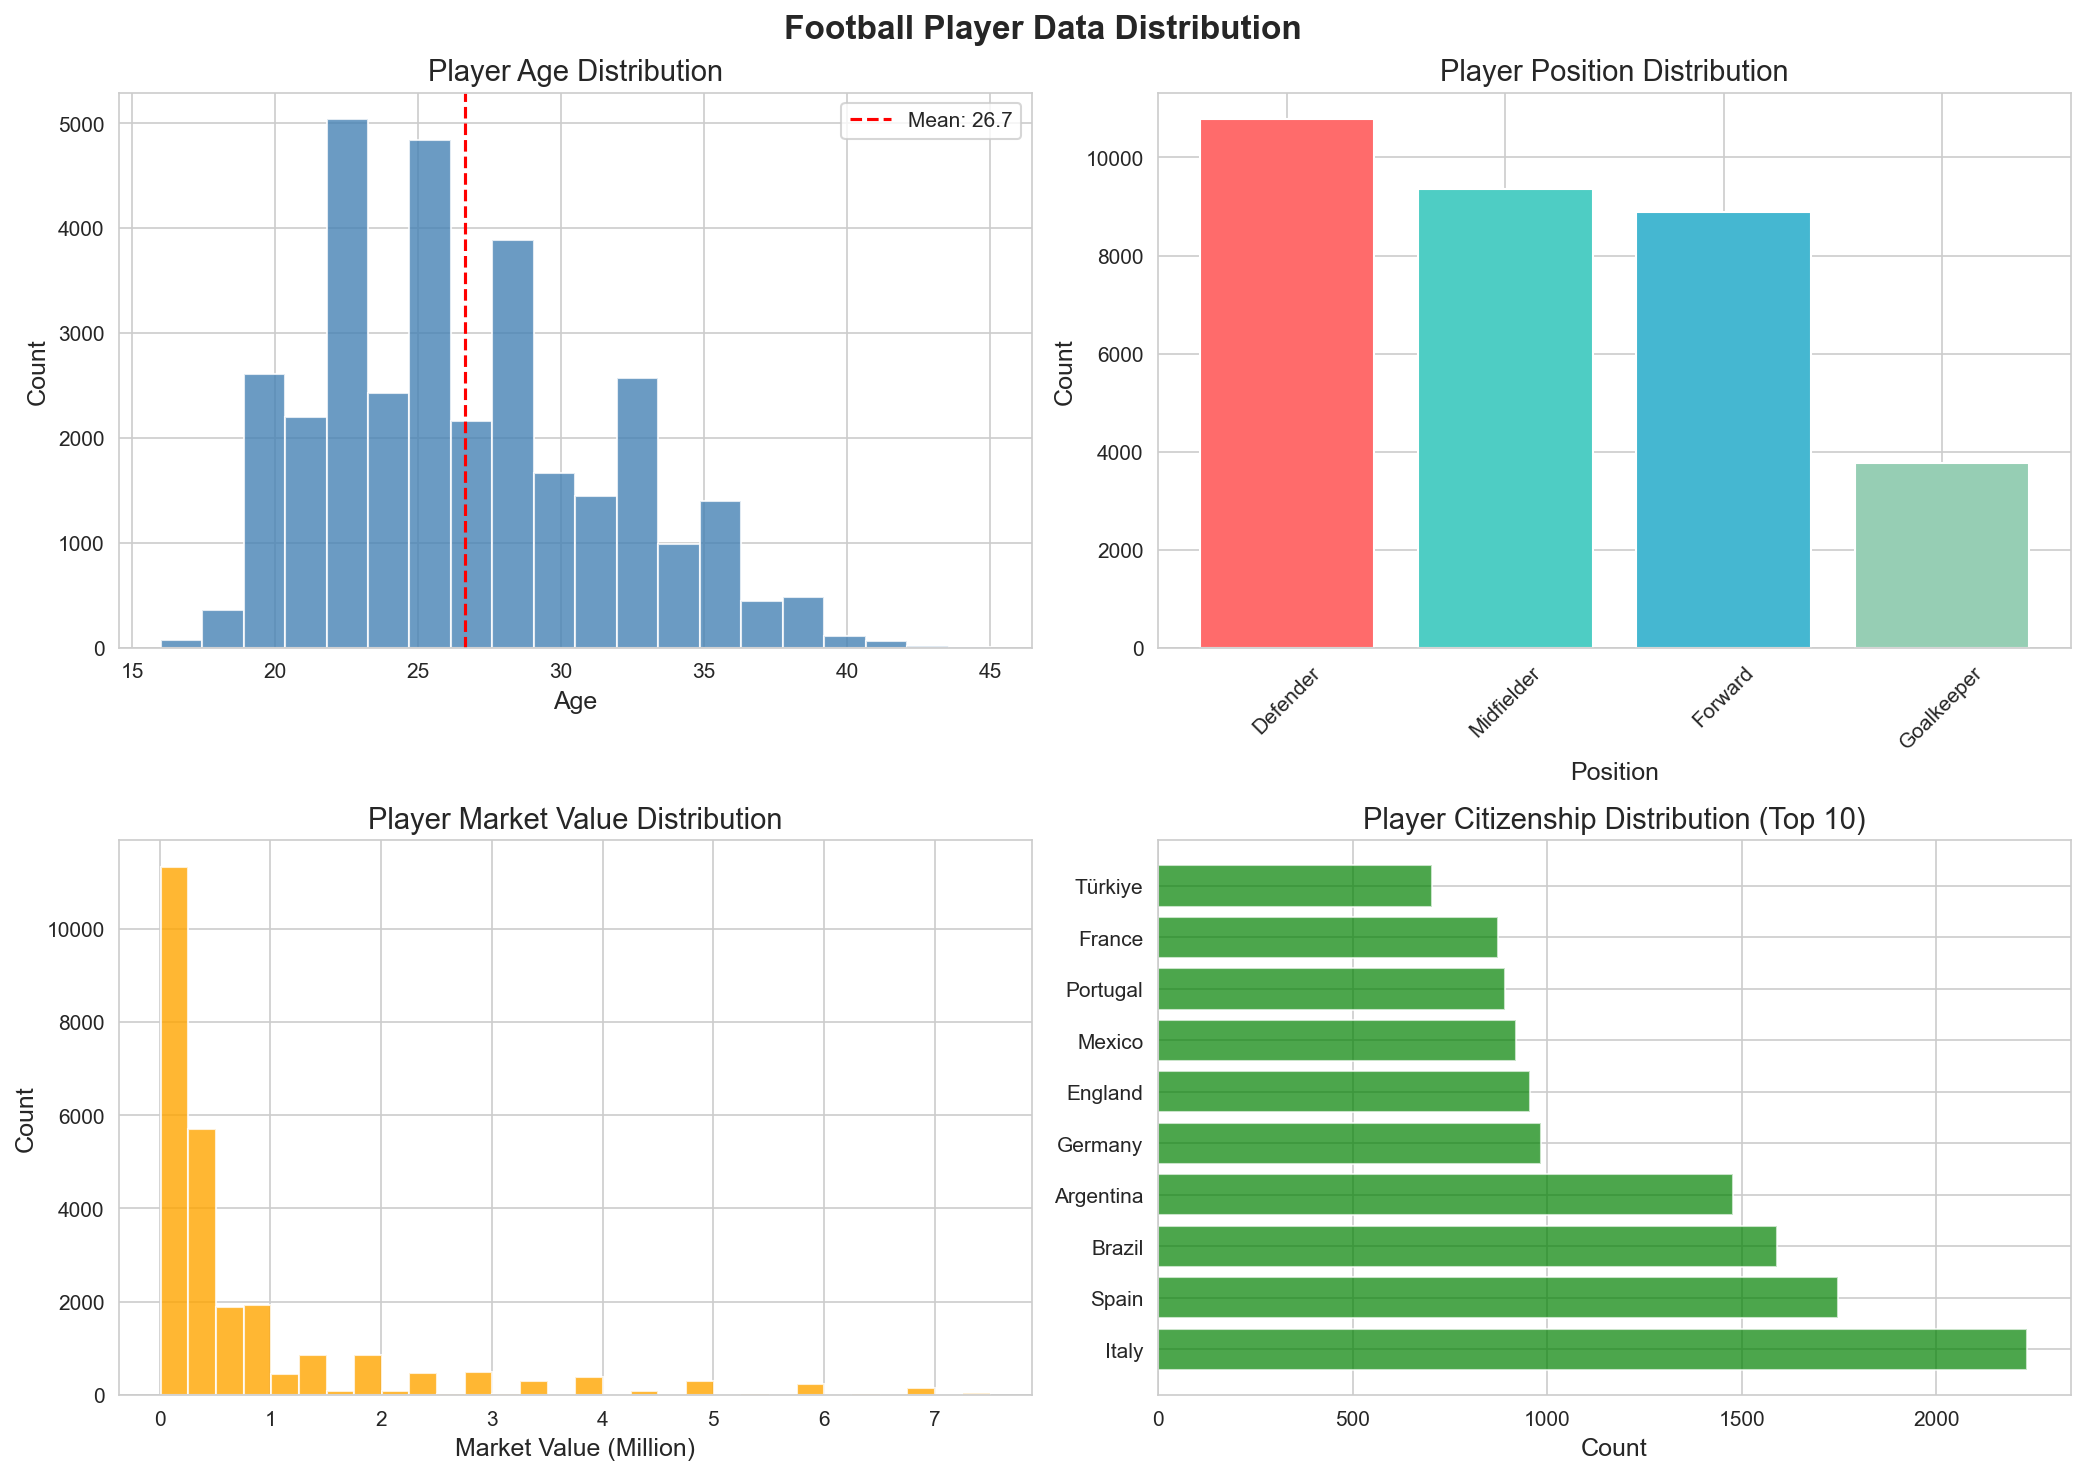
\includegraphics[width=0.75\textwidth]{img/player_distribution.png}
\caption{球员分布图。展示了球员在不同维度的分布特征，包括年龄分布直方图、身价分布密度图以及俱乐部球员数量分布。年龄分布呈现右偏态，峰值集中在24-28岁；身价分布呈现典型的长尾分布（幂律分布），绝大多数球员身价集中在较低区间，仅少数顶级球星拥有极高身价。俱乐部球员规模方面，大部分俱乐部的一线队人数集中在20-30人之间。}
\label{fig:player_dist}
\end{figure}

\begin{figure}[H]
\centering
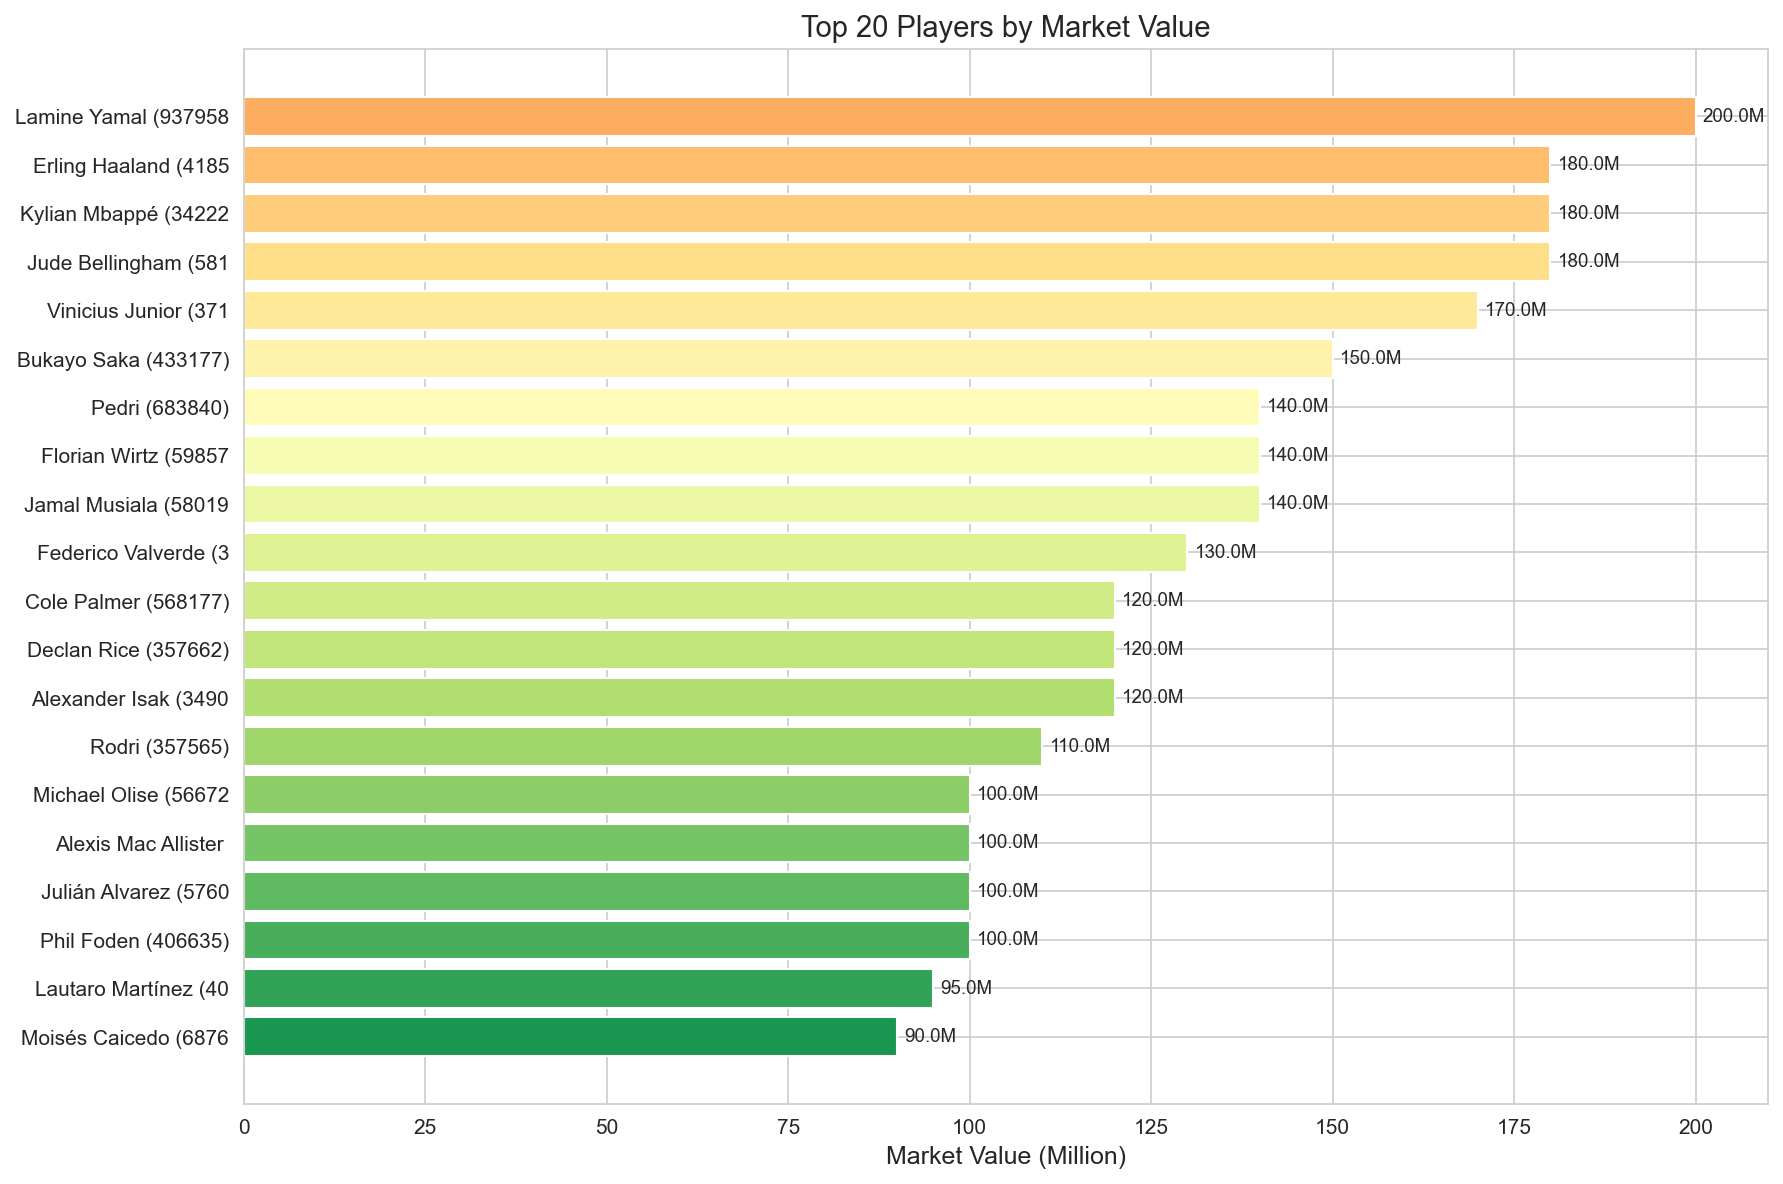
\includegraphics[width=0.7\textwidth]{img/top_players.png}
\caption{高身价球员统计图。展示了身价排名前20位的球员信息，包括姓名、所属俱乐部和身价（百万欧元）。Top 5球员分别为Lamine Yamal（200M\texteuro{}）、Erling Haaland（180M\texteuro{}）、Kylian Mbappé（180M\texteuro{}）、Jude Bellingham（180M\texteuro{}）和Vinicius Junior（170M\texteuro{}），反映了当前足球转会市场上年轻攻击型球员（尤其是前锋和攻击型中场）的极高商业价值。这一数据也间接说明了为什么基于流行度（身价）的冷启动策略在某些场景下仍有参考意义。}
\label{fig:top_players}
\end{figure}

\subsection{Web 演示系统 (Demo) 展示}

为了直观展示推荐系统的核心功能与创新点，团队基于 Flask 框架开发了一套 Web 演示界面，支持球队分析与需求感知推荐、相似球员推荐两大核心模式。

\subsubsection{球队分析与需求感知推荐}

\begin{figure}[H]
\centering
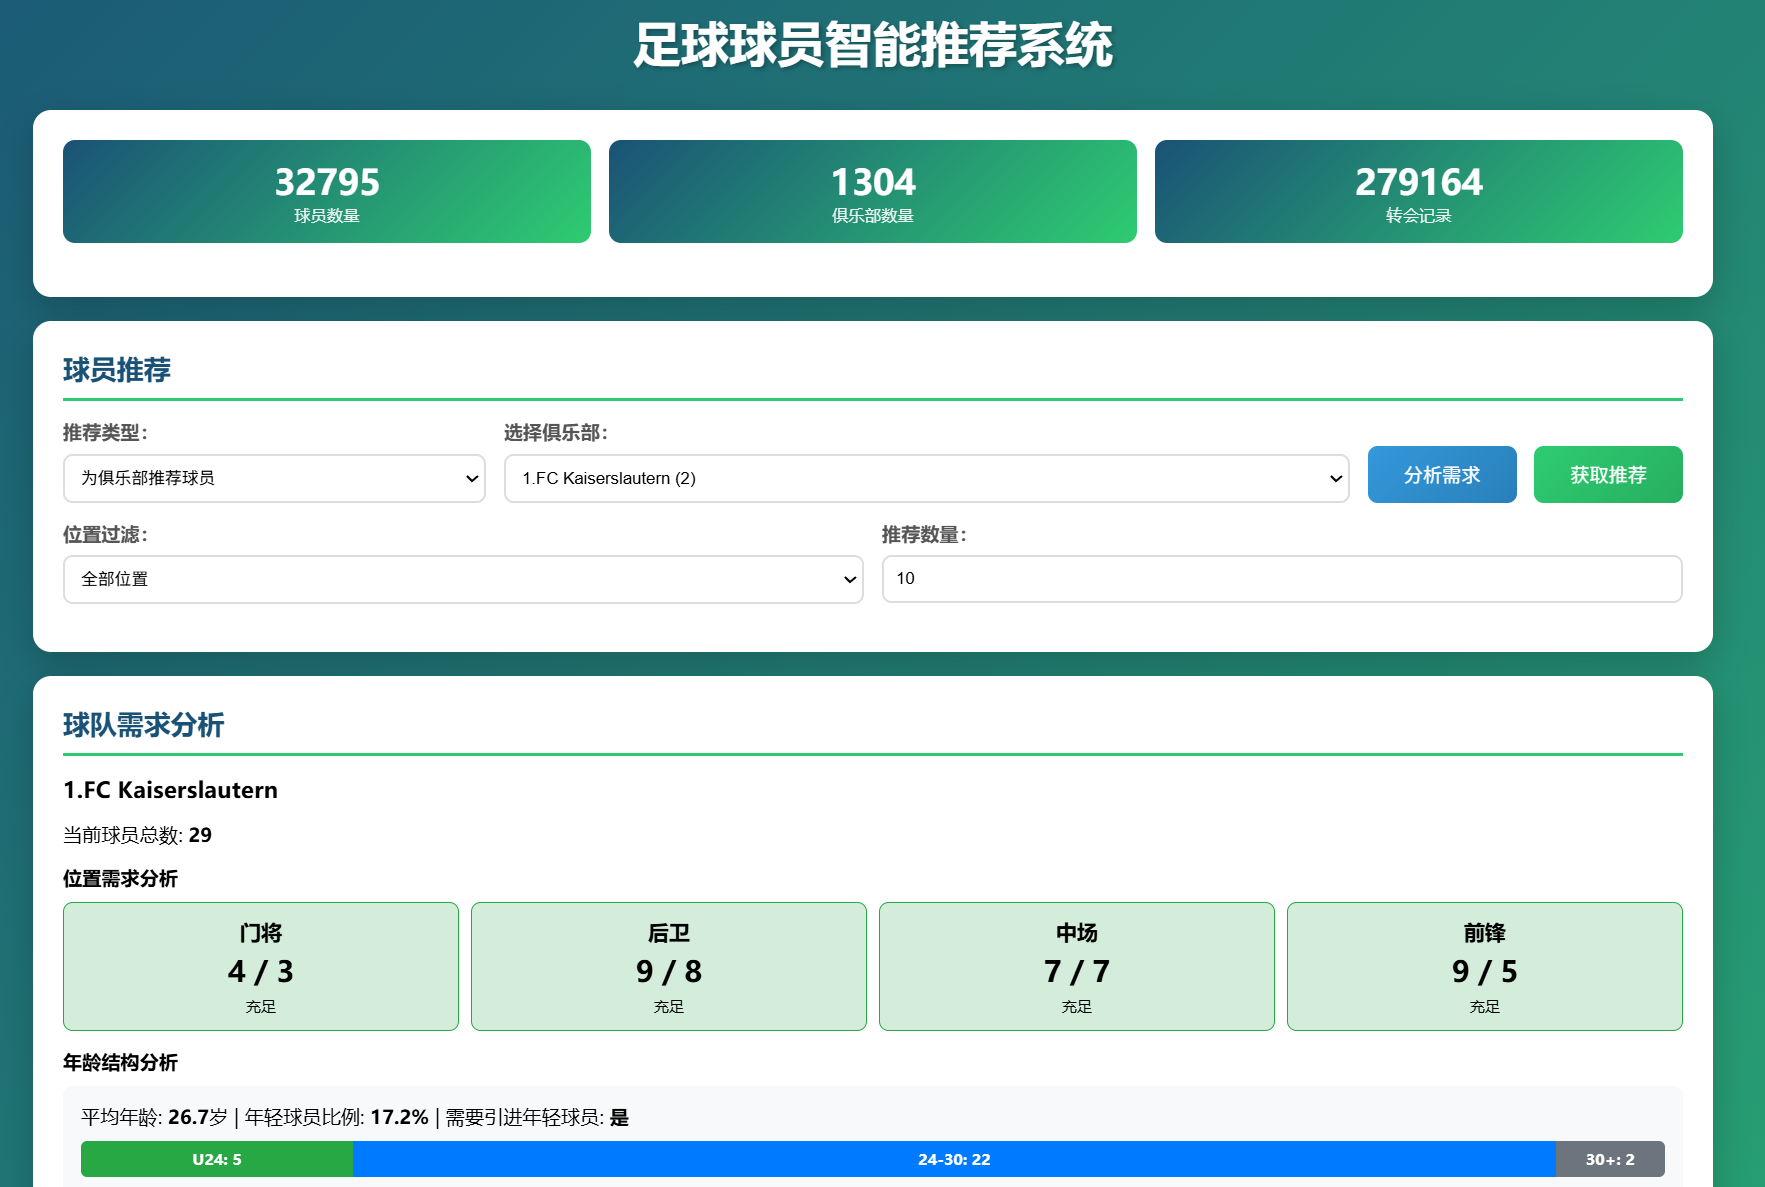
\includegraphics[width=0.7\textwidth]{img/demo1.png}
\caption{需求感知推荐——阵容缺口分析界面。用户选择目标俱乐部后，系统自动生成该俱乐部当前各位置的球员数量分布，并与理想阵容配置（门将3人/后卫8人/中场7人/前锋5人）进行对比。图中清晰标示了各位置的缺口状态（红色高亮表示严重不足、黄色表示略缺、绿色表示充足）。}
\label{fig:demo1}
\end{figure}

\begin{figure}[H]
\centering
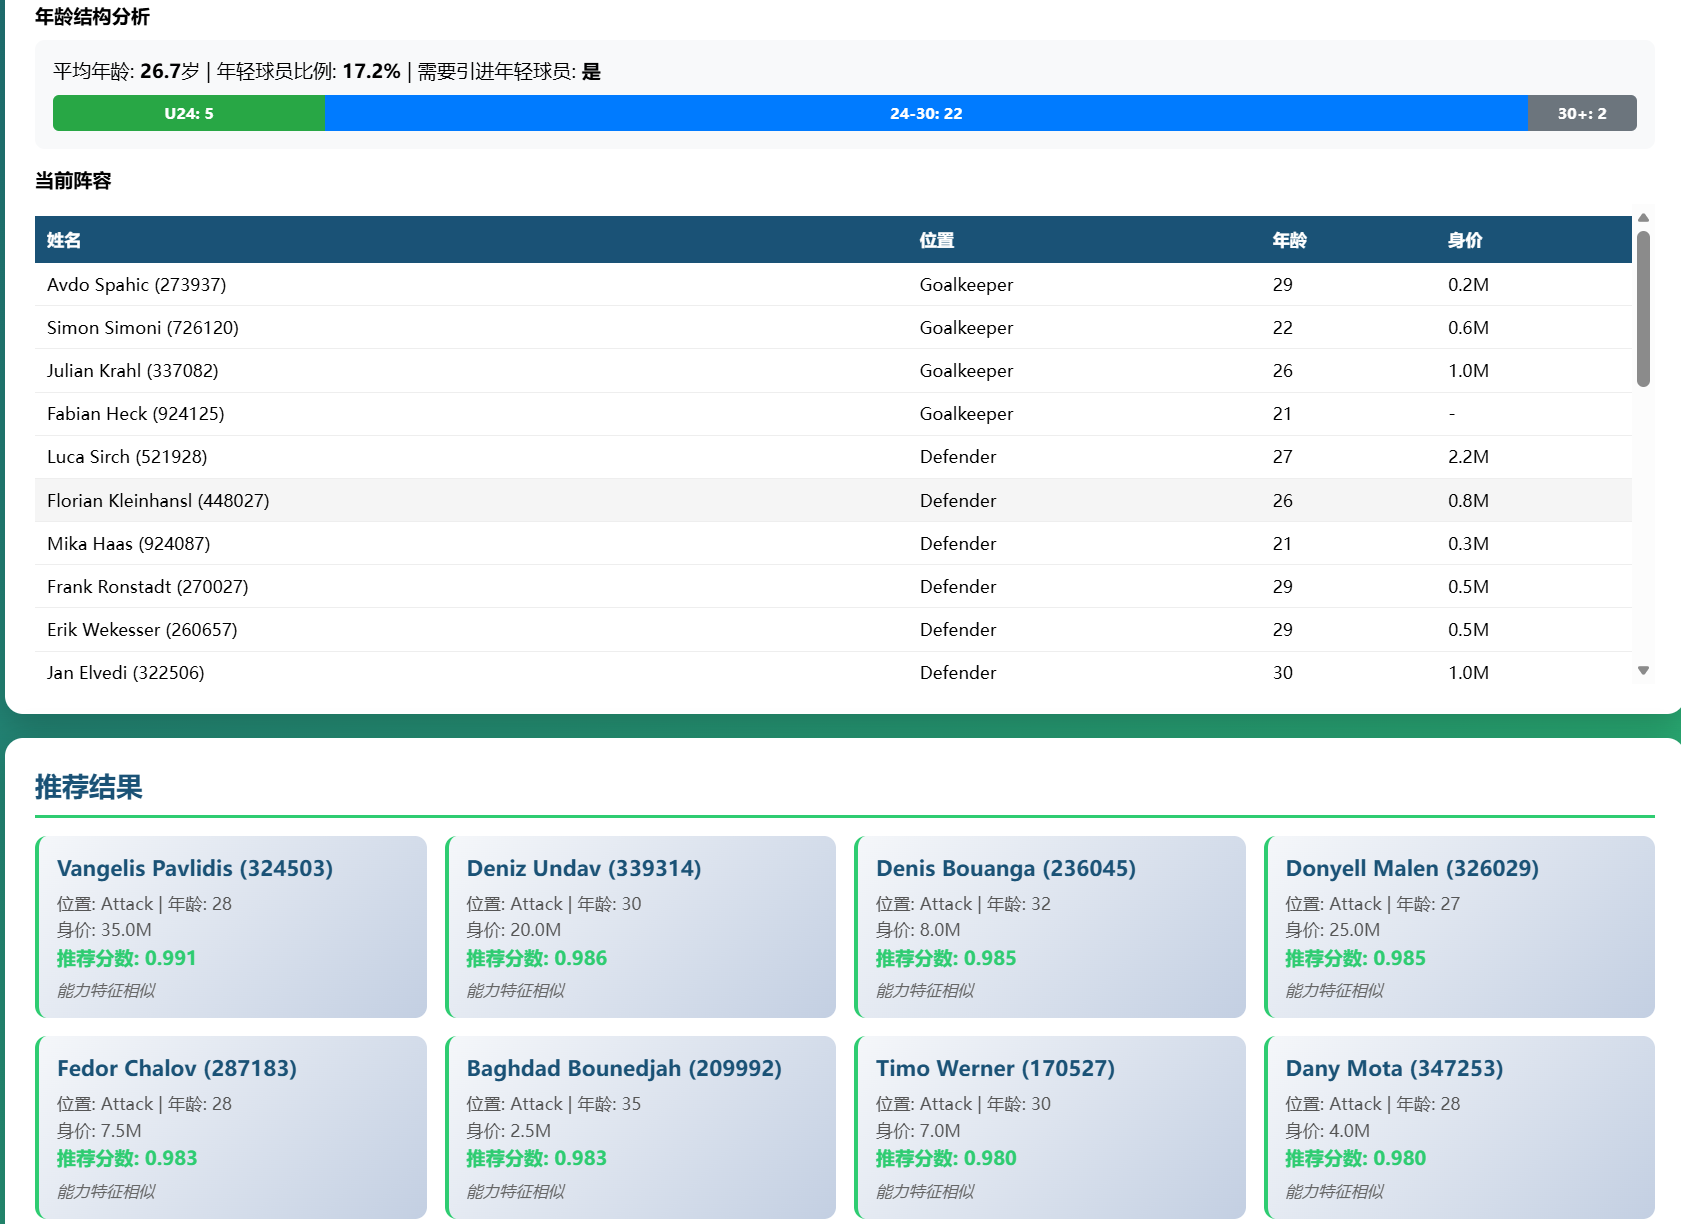
\includegraphics[width=0.95\textwidth]{img/demo2.png}
\caption{需求感知推荐——年龄结构分析与推荐结果。基于阵容缺口分析结果，系统进一步展示该俱乐部的年龄结构可视化柱状图（按 U24 / 24--28 / 28--30 / 30--32 / 32+ 分组），并通过自定义逻辑判断球队是否面临阵容老化风险。推荐列表中的每位球员均以卡片形式呈现，包含姓名、位置、年龄、身价等关键信息，并按照融合后的综合得分进行排序——位置匹配合格且年龄符合结构调整需求的球员将获得更高的展示排名。}
\label{fig:demo2}
\end{figure}

上述两张截图完整展示了系统的核心创新工作流：从俱乐部的阵容现状诊断（位置缺口、年龄结构）到需求感知的个性化推荐结果生成，形成一个闭环的智能引援辅助决策链。

\subsubsection{相似球员推荐}

\begin{figure}[H]
\centering
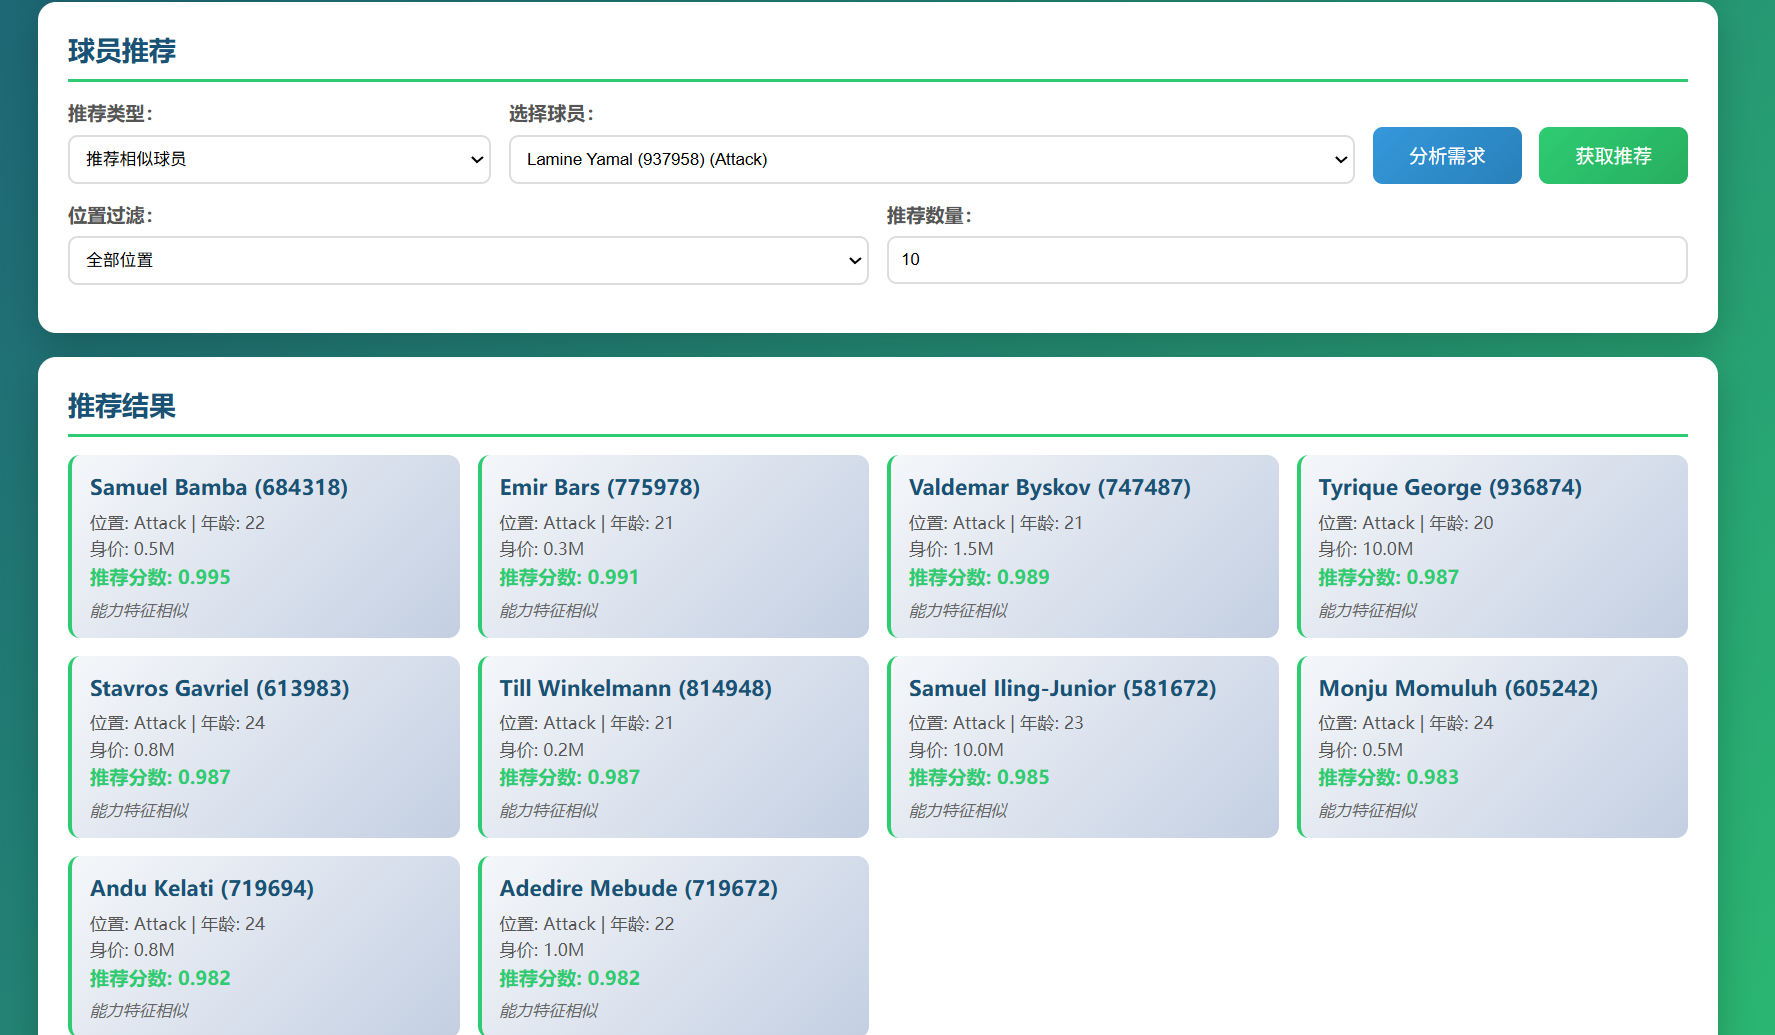
\includegraphics[width=0.95\textwidth]{img/demo3.png}
\caption{相似球员推荐模式。通过输入特定目标球员姓名（示例中为 Lamine Yamal），系统调用 Content-Based 模块提取该球员的多维度特征向量（比赛能力统计、身价、位置编码等），在整个球员候选池中计算余弦相似度，并返回相似度得分最高的 Top-K 候选人。图中展示的推荐结果均附有具体的相似度得分，便于俱乐部球探快速评估每位候选人与目标球员的综合平替价值。这一功能在球探寻找转会目标的高性价比替代方案时具有显著的实用价值。}
\label{fig:demo3}
\end{figure}

相似球员推荐模式为足球转会市场中的"平替球员挖掘"场景提供了算法支持——当目标球员因身价过高或合同受限无法签下时，系统可以快速从全球球员池中检索出能力特征高度相似但身价更合理的替代候选人，有效辅助俱乐部做出更经济的引援决策。


% ============================================================
% 5. 实验总结
% ============================================================
\section{实验总结}

\subsection{主要收获}

通过本次大数据原理与技术课程大作业的实践，团队在以下方面取得了显著收获：

\begin{enumerate}
    \item \textbf{推荐系统工程实践能力的全面提升}：从数据集的调研选型、数据清洗与特征工程，到协同过滤、基于内容推荐、混合推荐算法的实现与评估，再到Web演示界面的开发，团队成员完整经历了一个大数据推荐系统从零到一的全流程构建。这一过程不仅加深了对课堂理论知识的理解，更培养了解决实际工程问题的综合能力。
    
    \item \textbf{领域知识与算法创新的深度融合}：足球领域的特殊性（位置体系、年龄结构、转会市场规律）为推荐算法的设计提供了独特的约束和创新空间。团队提出的"阵容缺口感知"和"多维度相似度融合"两项创新点，正是在深入理解足球领域特征的基础上，对通用推荐算法进行领域适配的产物。实验数据充分证明，领域知识驱动的算法设计能够带来显著的性能提升。
    
    \item \textbf{冷启动问题的应对策略}：在俱乐部协同过滤中，大量俱乐部仅有少量转会记录，面临严重的冷启动问题。团队采用了"基于流行度的退化策略"作为冷启动的fallback方案——当目标俱乐部缺乏足够的协同过滤信号时，自动切换为按球员身价排序的流行度推荐。虽然这一策略的个性化程度有限，但在数据极度稀疏的场景下，仍能提供具有一定参考价值的推荐结果。
    
    \item \textbf{多维评估体系的重要性}：传统推荐系统评估往往过度关注准确率指标（Precision、Recall），但本实验通过引入Coverage、Diversity和领域特定的"位置需求满足度"，形成了更为全面的评估体系。实验结果表明，准确率指标与覆盖度/多样性指标之间存在一定的权衡关系，单一维度的评估无法全面反映推荐系统的实际效用。
\end{enumerate}

\subsection{存在的不足与改进方向}

尽管本系统取得了较好的实验结果，但仍存在若干局限性和改进空间：

\begin{enumerate}
    \item \textbf{特征维度有待扩展}：当前特征工程主要依赖球员的比赛表现统计（进球、助攻、出场时间等），尚未充分利用数据集中的伤病记录（player\_injuries）和球员国家队表现（player\_national\_performances）等信息。引入伤病历史可以帮助评估球员的出勤可靠性，引入国家队表现可以提供更高水平比赛的参考数据。此外，比赛事件级别的细粒度数据（如传球成功率、抢断次数、跑动距离等）若能获取，将极大丰富球员能力画像的精度。
    
    \item \textbf{转会预算约束的缺失}：当前推荐系统未考虑俱乐部的转会预算限制。在实际转会决策中，球员身价与俱乐部预算的匹配是硬性约束条件。未来可以在推荐流程中增加预算过滤模块，或引入多目标优化框架，在推荐准确性和预算可行性之间寻求最优平衡。
    
    \item \textbf{深度学习模型的引入}：当前系统完全基于传统机器学习方法（余弦相似度、协同过滤），尚未尝试深度学习方法。图神经网络（Graph Neural Networks, GNN）在球员-俱乐部关系建模方面具有天然优势——可以将球员、俱乐部、转会关系建模为异构图，通过消息传递机制学习节点的低维嵌入表示，有望在推荐精度和泛化能力上实现新的突破。
    
    \item \textbf{实时数据更新能力}：当前系统的数据处理和模型训练均为离线批处理模式。在实际应用中，球员身价、比赛表现和转会信息持续更新，需要系统具备增量更新或在线学习能力，以保持推荐结果的时效性。

\end{enumerate}

\end{document}